% Puede generar borradores si omite la opción "final" de la clase.
% \documentclass{udpthesis}
\documentclass[final]{udpthesis}

% Establecemos el sistema para uso del español
% Babel ya esta cargado dentro de updthesis
\usepackage[T1]{fontenc}%    output
\usepackage[utf8]{inputenc}% input
\usepackage{calc}
\usepackage{ifthen}
\usepackage{lmodern}
\usepackage{listings}
\usepackage{tikz}
\usetikzlibrary{shapes,arrows}
\usepackage{verbatim}
\usepackage{nomencl}
\usepackage{pgfplots} % fuer plots
\usepackage[external]{forest}



% Leyendas
\usepackage[font=footnotesize,labelfont=bf,labelsep=period]{caption}

% Agregue acá otros paquetes que le sean de utilidad
\usepackage{amsmath}	% Matemáticas\bigtriangleup
\usepackage{graphicx}	% Gráficos
\usepackage[font=footnotesize,labelformat=simple]{subfig}
\usepackage[acronym]{glossaries}



\makeglossaries


\newglossaryentry{latex}
{
	name=latex,
	description={Is a mark up language specially suited for 
		scientific documents}
}

\newglossaryentry{maths}
{
	name=mathematics,
	description={Mathematics is what mathematicians do}
}

\newglossaryentry{formula}
{
	name=formula,
	description={A mathematical expression}
}

\newacronym{gcd}{GCD}{Greatest Common Divisor}
\newacronym{lcm}{LCM}{Least Common Multiple}




% Cambiamos el formato de las leyendas: finalizan en punto, y en negrita.
\captionsetup{labelsep=period,labelfont=bf}

% Habilitamos el uso de paréntesis al citar las figuras con subfiguras dentro, e.g., Fig. 1(a)
\renewcommand\thesubfigure{(\alph{subfigure})}
\renewcommand\thesubtable{(\alph{subtable})}
\newcommand{\subfigureautorefname}{\figureautorefname}


\lstset{
 % language=[LaTeX]TeX,
 breaklines=true,
 basicstyle=\tt\scriptsize,
 keywordstyle=\color{blue},
 identifierstyle=\color{black},
 commentstyle=\color{green!40!black},
 % frame 
 frame=tb,
 captionpos=t,
 xleftmargin=1em,
 numbersep=0.3em,
 % numbers=left,
 framexleftmargin=1.1em,
 framexrightmargin=0pt,
 % additional letters for accents in spanish
 literate=%
   {á}{{\'{a}}}1
   {é}{{\'{e}}}1
   {í}{{\'{i}}}1
   {ó}{{\'{o}}}1
   {ú}{{\'{u}}}1
   {ñ}{{\~{n}}}1
   {Ñ}{{\~{N}}}1
}


% Código
% Para generar código fuente usar listings.sty
%\usepackage{listings}
%\usepackage{tikz}
%\lstset{
%  language=[LaTeX]TeX,
%  breaklines=true,
%  basicstyle=\tt\scriptsize,
%  keywordstyle=\color{blue},
%  identifierstyle=\color{magenta},
%  commentstyle=\color{green!40!black},
%  % frame 
%  frame=tb,
%  captionpos=t,
%  xleftmargin=1em,
%  numbersep=0.3em,
%  numbers=left,
%  framexleftmargin=1.1em,
%  framexrightmargin=0pt,
%  % additional letters for accents in spanish
%  literate=%
%    {á}{{\'{a}}}1
%    {é}{{\'{e}}}1
%    {í}{{\'{i}}}1
%    {ó}{{\'{o}}}1
%    {ú}{{\'{u}}}1
%    {ñ}{{\~{n}}}1
%    {Ñ}{{\~{N}}}1
%}
%
%\renewcommand{\lstlistingname}{Código}% Listing -> Código
%\DeclareCaptionFormat{listing}{\rule{\dimexpr\linewidth\relax}{0.4pt}\par\vskip1pt#1#2#3}
%\captionsetup[lstlisting]{format=listing,singlelinecheck=false, margin=0pt,position=bottom}

% O para generar algoritmos en pseudocódigo usar algpseudocode.sty
\usepackage{algorithm}% http://ctan.org/pkg/algorithms
\usepackage{algpseudocode}




%\makeatletter
%\renewcommand{\ALG@name}{Algoritmo}% Algorithm -> Algoritmo
%\makeatother
%\captionsetup[algorithm]{font=footnotesize,labelsep=period}

\usepackage{cite}% Referencias (este paquete ordena y comprime las referencias)


\udptheme{EIT}


\begin{document}




\frontmatter %% Inicio de la portada

\title{Modelo de Predicción Secuencial de Webaccess Log basado en un Algoritmo de Compresión y Machine Learning}

% para precisar aún más su tema, use un subtítulo
%\subtitle{Subtítulo explicativo del tema}
\author{Jaime Guzmán}
\email{mail@jguzman.cl}
\date{2015}


% Profesor guía
\professor{Adín Ramirez}
% Comité
\committee{Francisco Claude}{Roberto Konow}

% Dedicatoria
\dedicatory{Dedicado a mi hijo, mis Padres y las personas que no dejaron de apoyarme a pesar de las adversidades.}

% Agradecimientos
%\acknowledgment{ % Nota redactada sobriamente en la cual se agradece a quienes han colaborado en la elaboración del trabajo. No puede exceder más de una página.

Mis primeras palabras de dedicatoria  y gratitud son para mi hijo Julian, mi hermano y mis padres, sin su apoyo incondicional en las buenas o malas decisiones que he tomado, siempre han estado para apoyarme, tal vez nunca hubiera podido terminar esto con el ritmo del trabajo y el estudio, pero ustedes siempre me motivaron, al igual que mi hermano.  Javier muchas gracias por ser mi más grande referencia en este mundo académico, espero presentar antes que termine su doctorado en Boston. También debo agradecer a mis trabajos que me han permitido financiar y lograr llegar hasta aquí, que ha costado mucho, muchas gracias  por ayudarme con el tiempo y facilidades para poder afrontar ciertos momentos en los que ha sido complicado continuar. Inmensamente agradecido a  Felipe Hermosilla y Jorge Cañon (Bice Vida - compañía de seguros), Max Díaz y Felipe Hrdina (RLGroup SPA - RatslabsIO\footnote{\url{http://www.ratslabs.io}}).

También agradezco a mis mentores y profesores guías: Adín Ramirez y Francisco Claude. Adín por darme la disciplina y enseñarme a escribir rigurosamente documentación de investigación y llevarme siempre más allá de lo que me he propuesto, como también ayudándome a abordar este tema con sus puntos de vistas y basto conocimiento, muchas gracias por su paciencia infinita para recibirme y llamarme la atención cuando desaparecía. También ha Francisco Claude por iniciarme en estos temas y motivarme, como también por un ser un gran referente en los temas de interés que abordado, probablemente sin sus consejos nunca habría intentado tomar un tema como éste, muchas gracias a ambos, ustedes me han inspirado enormemente. 

Finalmente debo agradecer a la Universidad Diego Portales, a sus administrativos y profesores que he ido conociendo en él camino, sin orden particular: Ximena Geoffroy, muchas gracias por su paciencia para escucharme y aconsejarme en todo momento, Loreto Montenegro, J. Frez, Sergio Mujica, Martin Gutierrez, Javier Pereira, Diego Dujovne, Jorge Elliot, todos han contribuido a que me guste más lo que estudié y trabajo día a día. También a mis amigos que hice durante la carrera y fuera de la universidad, por comprenderme y darme mucho ánimo para finalizar este trabajo y por último, muchas gracias María Paz haz sido fundamental en este proceso. }

% Abstrat en inglés
\abstract{ Internet is growing every day and data volumes grow in the order of 
terabytes, for this reason it is of interest to use compression 
techniques for larger-scale processing of information with the fewest 
possible resources. Today there are various types of web: social networks, microbloging, web information, etc. The content provided to end 
users is not static and this allows them to create, contribute, and 
modify content, so Web Development Industry is constantly evolving to generate 
better solutions and friendly interaction with the users. 
Many of these new technologies have to deliver a better experience when browsing, the breakthrough has made it possible to create Web that are themselves intelligent and anticipating their behavior can go to, for example, decrease latency from a website and accessed or since navigate within a site with high concurrency; also from the point of view of the current web service patterns that are consumed immediately give a wide application area and provides a strategic aspect to the use of the information. While the growth of storage resources in the cloud is in full swing, networks don't grow at the same speed, which gives an area of interest to deepen.


So in this thesis we  propose the creation of a hybrid model between Machine Learning and Lossless Data Compression  for predict the next page that some user can access within a web; using training techniques and compression algorithms like well know \texttt{LZ78}, on a server Machine Learning. To this end we will work to create and study a predictive model that uses both areas and provide the results of the predictive model with integrated online component to any type of platform. }

% Resumen
\resumen{ 	%El resumen no debe contener menos de 100 palabras ni mas de 300 palabras.

Internet crece exponencialmente  y los datos son generados en grandes volúmenes, en el orden de los \emph{Terabytes}. Hoy en día existen varios tipos de \emph{webs}: redes sociales, microbloging, \emph{web} informativas, etc. esto genera un interés en usar técnicas de compresión para realizar procesamiento a mayor escala de información con la menor cantidad de recursos posibles. El contenido proporcionado a los usuarios finales ya no es estático y esto permite que los mismos puedan  aportar, modificar ó eliminar contenido. Así  la industria del desarrollo web está en constante evolución para generar más variados recursos para ser usados. Muchas de estas nuevas tecnologías han permitido entregar mejor experiencia al momento de navegar en el lado del cliente, pero el gran avance realizado aún no permite crear \emph{web} que sean en sí inteligente por si misma y pueda ir anticipando la  navegación de un usuario o la recomendación de un contenido, tenemos los siguientes ejemplos; disminuir la latencia desde que se comienza a navegar una \emph{web} prediciendo los accesos futuros del usuario o aún mejor reconocer patrones discretos en la navegación de un usuario,  de un sitio concurrente; también desde el enfoque de los patrones de desarrollo \emph{web} actuales, los servicio  se consumen inmediatamente y dan una área de aplicación e integración extensa, aportando un aspecto estratégico al uso de la información con procesamiento inmediato. Si bien el crecimiento del almacenamiento de datos en la nube se encuentra en auge en la industria, las redes de telecomunicaciones  no crecen a la misma velocidad, lo cual genera un campo de interés para investigar. 

En este trabajo proponemos  la creación de un modelo híbrido entre \emph{Machine Learning} y Algoritmos de tipo \emph{Lossless Data Compression} para predecir la siguiente secuencias de acceso que usuario puede realizará dentro en una web; usando un modelo de navegación basado en un Algoritmo de Compresión como \texttt{LZ78}, sobre un servidor de Machine Learning. Con este propósito se trabajará para crear y estudiar un modelo predictivo que use ambas áreas y  ofrezca los resultados del modelo predictivo con una componente \emph{online} integrable a cualquier tipo de plataforma cliente. }


\makecover			% Generamos la portada
\tableofcontents	% tabla de contenido
\listoftables		% Indice de tablas
\listoffigures		% Indice de figuras
\mainmatter			% Inicio del contenido


\chapter[Introducción]{Introducción}
\label{ch:intro}

%chacharara
{

Los nuevos avances tecnológicos  y la inclusión de la ciencia de la computación en distintas campos han permitido hacer colecciones de datos muy grandes, las cuales se deben procesar, clasificar y analizar. Encontrar información útil dentro de estos grandes volúmenes de datos significa poder mejorar la decisiones a las que se pueden tomar dada a una base de conocimiento.

La minería de datos basado en web access se ha convertido en un área importante de investigación en los últimos años. Se puede utilizar para mejorar el rendimiento de la caché web, la detección de intereses de los usuarios y así recomendar páginas o bienes relacionados para los sitios web de comercio electrónico, mejorar los resultados de los motores de búsqueda  y por ejemplo personalizar el contenido de la web con las preferencias deseadas para el usuarios . En la predicción de navegación web logrando entender el patrón de navegación del usuario y luego la predicción de las páginas siguientes es el principal problema que buscamos solucionar. Con un sistema de predicción fiable podemos ver la siguiente acción de los usuarios de Internet y tomar acciones.

Normalmente se ocupa muchos algoritmos de Machine Learning para poder hacer predicciones en variadas áreas.  Hoy en día las aplicaciones en que los usuarios se enfrentan no pueden ser estáticas y sin tener un comportamiento que ayuden a predecir la forma en que actúan los usuarios. Esta área toma mucha relevancia al encontrarnos en una auge de la información generada por usuarios, redes sociales y variadas plataformas. Podemos mencionar que esta es una de las razones para poder requerir disponer de herramientas de análisis y predicción que nos permitan saber como se comporta usuarios sobre una web, conocer la frecuencia en que se accede a un recurso en Internet, etc.

El momento en que un usuario entre a un web se establece una conexión cliente-servidor. Una gran cantidad de servicios proporcionan datos de accesos de los usuarios que acceden, sobre estos mismos se puede realizar variadas investigaciones sobre como predecir cual es la siguiente página que podrá visitar.

%%%%%%Moghaddam_Kabir
Las predicciones en los registros de web access han atraído una atención significativa en los últimos años. Muchas técnicas de recuperación de datos  y algunos sistemas de personalización usan algoritmos de predicción. La mayoría de las aplicaciones actuales que predicen la siguiente página Web de un usuario tienen una componente en línea que hace la tarea de preparación de datos y una sección en línea que proporciona contenido personalizado a los usuarios en función de sus actividades de navegación actuales. En este trabajo se presenta un modelo de predicción en línea que se puede consumir como un servicio de API el cual da una integración ha variadas plataformas y sistemas que no tenga un componente en línea y con una buena precisión de la predicción. 
Nuestro algoritmo se basa en algoritmos LZ78 que están adaptados para modelar  y representar la navegación secuencia del usuario en una web. Nuestro modelo disminuye la complejidad computacional, que es un problema grave en el desarrollo de sistemas de predicción en línea. 


  }

%%%%%%Moghaddam_Kabir
%Web access prediction has attracted significant attention in recent years. Web prefetching and some personalization systems use prediction algorithms. Most current applications that predict the next user web page have an offline component that does the data preparation task and an online section that provides personalized content to the users based on their current navigational activities. In this paper we present an online prediction model that does not have an offline component and fit in the memory with good prediction accuracy. Our algorithm is based on LZ78 and LZW algorithms that are adapted for modeling the user navigation in web. Our model decreases computational complexities which is a serious problem in developing online prediction systems. A performance evaluation is presented using real web logs. This evaluation shows that our model needs much less memory than PPM family of algorithms with good prediction accuracy.

%Web mining has become an important research area in recent years. It can be used to improve the web cache performance[1, 2], Detecting the user interests and so recommending related pages or goods for e-commerce web sites [3], improving search engines results [4] , and personalizing the web content as the users like [5]. In web page prediction understanding the user navigation pattern and then predicting the next pages is the main problem. With a reliable prediction system we can see the next action of web users.






%When user requests inserted and deleted incrementally the online models are desirable. In this paper we present efficient techniques for modeling user navigation behavior. Our model is online so changes in user request patterns will update our prediction model incrementally.
%%%%%%%%%%%%%%%%

% 

% Nuestro intere es hacer que las rpecicciones sean modeladas por un compresaor de datos basado en Lempel ziv



%%%%%%%%%%
% Uno de los interes en poder crear un un aplicación de ambas areas es la convergenia de las areas en la cual un proceso de aprendizaje ó predicción secuencial se puede usar con ML y Compress data
% Cuando se hace el pio train se hace un entrenamiento de modelo lo que resulta ser es que genera el arbol que es un trie de LZ que será el predicto
% Una función de predición implementada con MLIB y PIO sería predict () en scala




%%%%%%% CONTEXTO PRELIMINAR 
\section{Contexto preliminar} 
\label{sec:preliminar}

% Idealmente aca explicar el problema

  La Web crece constantemente y por ende su infraestructura, también la información que podemos obtener de los  usuarios y  por consecuencia mayor concurrencia de los sistemas, la cual para los usuarios finales se traduce en un incremento de latencia y una mejor o peor experiencia de usuario. Paralelamente se suma un costo exponencial de recursos tanto en tecnologías de desarrollo como servicio que no son optimizados para poder dar una experiencia de usuario con calidad de servicio. Podemos reflexionar, entonces, que tener mayores recursos no mejorará el rendimiento, ni tampoco será lo óptimo para dar una calidad de servicio web ya que el ancho de banda de Internet no crecerá en la misma proporción.
   
  Adicionalmente, las tecnologías para la creación de web dinámicas y asíncronas han evolucionado a favor de traspasar la carga cliente.
  Hoy en día ya se poseen lenguajes y {framework} que disminuyen considerablemente la carga de un servidor, por lo cual, un buen servicio web es proveer una balanceada carga dentro del cliente y el servidor, pero cuando se poseen un gran volumen de datos es fundamental tomar decisiones que los recursos y lenguajes no cubren, es ahí el interés de dar inteligencia a servicios de la web.

  Interpretaremos que la manera en que un usuario navega es su comportamiento o patrón registrado en \emph{webacces log}, y que se pueden analizar, estudiar y modelar con algoritmos que tengan enfoques predictivos. 

  Sobre estos registros se pueden hacer representaciones eficientes como las realizadas por Claude \etal~\cite{Claude2014},  minería de datos para buscar \emph{Web Usage Mining} (WUM), el porque de hacer minería de datos radica en que cada día la web genera una innumerable cantidad de información, por lo cual usar algoritmos que se puedan opera de manera comprimida o con una representación lo más liviana posible es de interés ya que además de disminuir el espacio físico o recursos utilizados, se puede usar como un algoritmo de predicción y trabajar con una mayor cantidad de datos.
  
  Teniendo el conocimiento que los \emph{webaccess logs} se pueden estudiar de manera procesada o pre-procesada, ayudaría a ingenieros de desarrollo web y diseñadores de experiencia de usuarios, como también en general a mejorar la experiencia de usuario final, también disminuyendo por ejemplo la latencia en respuestas por parte de cada petición realizada, con técnicas de \emph{pre-fetching predictivo} en el lado del cliente.
  

  Actualmente, los sitios web han evolucionado de ser contenido estático a dinámico, también moderado por administradores a contenido orgánico creado por usuarios finales. Se debe poseer una adaptabilidad a la demanda o proveer información que permita adaptarse a los eventos, por lo tanto, hacer un estudio sobre esto y poder hacer integraciones en áreas como uso de algoritmos de compresión y \emph{Machine Learning} presenta un gran desafío. Independientemente del área, el problema común  se puede resolver pero se busca encontrar las fortalezas de cada área y usarlas en conjunto. 

  Durante este trabajo se usarán técnicas de compresión de datos, se utilizará una infraestructura y patrón de implementación para modelos de \emph{Machine Learning} como servicio. Adicionalmente toda la experimentación se llevará acabo ofreciendo los algoritmos y modelos como servicio basado en una Transferencia de Estado Representacional (\emph{REST}~\ref{concept-rest}), y así implementarlo en áreas productivas las cuales pueden presentar interés dando nuevos escenarios de estudio.


  La sesión de un usuario comienza cuando se conecta a un servicio web, éstas pueden ser páginas informativas, redes sociales, web dinámicas, contenido colaborativo, etc. Estableciendo dicha conexión a una página, se crea en ese momento una sesión de navegación automáticamente. Dado esto es posible almacenar datos muy relevantes los cuales son ''webaccess log'' ó registros de accesos web, durante el texto se mantendrán las referencias en inglés. Un ejemplo de \emph{webaccess log} es lo que se observa en la figura ~\ref{fig-ejemplo-webaccesslogbruto}:

\begin{figure}[tb]\label{fig-ejemplo-webaccesslogbruto} 
	\centering
	\begin{lstlisting}[frame=single,basicstyle=\ttfamily\tiny,]
	172.31.33.116 - - [26/Nov/2015:00:12:12 +0000] "HTTP/1.1" 200 1784 "http://localhost/home" 
	"Mozilla/5.0 (Linux; Android 5.1.1; SAMSUNG SM-G920I Build/LMY47X) 
	SamsungBrowser/3.2 Chrome/38.0.2125.102 Mobile Safari/537.36"
	172.31.33.116 - - [26/Nov/2015:00:12:12 +0000] "HTTP/1.1" 200 179333 "http://localhost/news" 
	"Mozilla/5.0 (Linux; Android 5.1.1; SAMSUNG SM-G920I Build/LMY47X) 
	SamsungBrowser/3.2 Chrome/38.0.2125.102 Mobile Safari/537.36"
	172.31.33.116 - - [26/Nov/2015:00:12:12 +0000] "HTTP/1.1" 200 24660 "http://localhost/health" 
	"Mozilla/5.0 (Linux; Android 5.1.1; SAMSUNG SM-G920I Build/LMY47X) 
	SamsungBrowser/3.2 Chrome/38.0.2125.102 Mobile Safari/537.36"
	172.31.33.116 - - [26/Nov/2015:00:15:12 +0000] "HTTP/1.1" 200 24604 "http://localhost/sports" 
	"Mozilla/5.0 (Linux; Android 5.1.1; SAMSUNG SM-G920I Build/LMY47X) 
	SamsungBrowser/3.2 Chrome/38.0.2125.102 Mobile Safari/537.36"
	172.31.33.116 - - [26/Nov/2015:00:20:12 +0000] "HTTP/1.1" 200 4860 "http://localhost/home" 
	"Mozilla/5.0 (Linux; Android 5.1.1; SAMSUNG SM-G920I Build/LMY47X) 
	SamsungBrowser/3.2 Chrome/38.0.2125.102 Mobile Safari/537.36"
	172.31.33.116 - - [26/Nov/2015:00:22:19 +0000] "HTTP/1.1" 200 4841 "http://localhost/finances" 
	\end{lstlisting}
	
	
	
	\caption{Ejemplo de un \emph{webaccess Log} de un servidor Apache.}
	\label{fig:accesslog-apache-teleton}
\end{figure}


  En la Figura \ref{fig-ejemplo-webaccesslogbruto} nos entrega mucha información interesante como la \texttt{IP} desde donde se conecta, el tipo de navegador, el dispositivo si es un teléfono inteligente o un navegador de escritorio, la fecha en que se realizó el acceso y también lo más relevante el destino del usuario.
  
  
  
  




\section{Definición del Problema}


El problema de la Predicción, ha surgido hace años y diversos investigadores han trabajado con distintos enfoques. Rissman y Langdom en los laboratorios Bell al realizar pruebas con un robot y hacer un experimento con un robot que tiraba una moneda compitiendo con humano, realizaba todos los calculos markovianos y calculos de las probabilidades condicionales para que cierto evento ocurra, a diferencia del sujeto que solo estaba esperando un resultado.

Predecir no es trivial, pero si podemos llegar a cercanos y minimizar el error de equivocarnos. Sin embargo, dos áreas han tratado de resolver el problema, LDC y Machine Learning de manera separada. Por parte de LDC los mayores problemas son que los predictores funcionan totalmente desconectados y no dan una de disponibilidad inmediata de los resultados, en cambios en el área de Machine Learning debemos crear un modelo para entrenar y luego poder generar una función predictiva.

Planteamos el problema de poder resolver tener un modelos híbrido juntando los patrones de cada área y disponerlo como un servicio inmediato dando una predictibilidad inmediata que hoy en la industria es necesaria para poder hacer útiles estos algoritmo y dar un valor a los avances.

 




% @TODO: SEGUIR TRABAJANDO EN ESTA BREVE INTRODUCCION
%En este tema convergen tres áreas, por un lado existe trabajo para crear estructuras eficientes para predicciones basadas en algoritmos de compresión, como es en el caso de~\cite{Claude2014}, y, por otro lado, el uso de algoritmos de aprendizaje para realizar clustering y predecir el comportamiento basado en el mismo contenido o en la distancia del contenido que visita el usuario actual al contenido clusterizado, como es el caso de ~\cite{Poornalatha2012}, inclusive se han utilizado modelos de Markov en ~\cite{Dongshan2002}  para poder modelar el comportamiento de la web.
%La tercera área son los Sistemas de Recomendación, la cual en este proyecto no se tocará pero si se mencionará el enfoque práctico que presenta área como un foco de múltiples implementaciones. 







%Algoritmos como serivcio
\section{Algoritmos como servicio web }

	Los avances en el desarrollo de nuevas tecnologías que brinden mejores experiencias en su uso día a día, deriva en cómo podamos llevar varios escenarios idealizados a implementaciones empresariales reales. Es bastante común encontrar librerías que son bastante útiles para hacer Minería de Datos, agrupación y muchas operaciones que pueden recurrir en cálculos muy complejos, pero no se pueden ofrecer como servicio. Ya en pleno auge de las infraestructuras en la nube, la capacidad de cómputo que se puede alcanzar no es un problema como antes lo era para un Científico de Datos.


	Una \emph{API} es un interfaz de programación de Aplicaciones que nos permiten intermediar el \emph{Servicio $A$} con el \emph{Servicio $B$}. Respectivamente $A$ puede ser el proveedor y $B$ el demandante del servicio. Si quisiéramos analizar datos que se encuentran dentro de un servidor específico, estos se podrían consumir por esta interfaz. Existen variados clientes que nos permiten ayudar en esta comunicación, incluso se pueden utilizar por una terminal de {Unix} que es posible dialogar mediante el programa \emph{curl}.
	
	Ya se dispone de infraestructura como servicio (\emph{IaaS}) , software como servicio (\emph{SaaS}), plataformas como servicios (\emph{PaaS}). Dado lo anterior ofrecer estos algoritmos para hacer que las soluciones de desarrollo den valor agregado a la experiencia requerida por el usuario final. Por esto hemos decidido utilizar una librería y {framework} que nos de esta posibilidad. Ofrecer algoritmos a la industria como un servicio que ayuda de manera eficiente e Inteligente desarrollado como una API REST, que permitirá una fácil integración. 
	
	Todas las ventajas de este patrón son heredados de las características que ofrece una API, interoperabilidad, evitar problemas de Infraestructura, Resiliencia de Datos, Persistencia de Datos, Análisis y Procesamiento sin afectar un curso operacional de una aplicación. Un ejemplo claro de esto es el análisis de datos en sistemas legados los cuales en plan de mejoras, no poseen la compatibilidad para poder realizarlo. Por otro lado, los algoritmos de compresión o algoritmos de \emph{Machine Learning} tienden a ser muy complejos de implementar o ocupan muchso recursos y este hecho pueden ser la razón para no implementarlos. 
	
	
	
	




%introducción a las Prediccion


\section{Predecir con \emph{PredictionIO}}

  	
En esta sección se presenta formalmente el ambiente de desarrollo que se utilizará durante este trabajo. \emph{PredictionIO} es un servidor de \emph{Machine Learning} de código abierto para Científico de Datos y Desarrolladores que permite crear motores de predicción para aplicaciones en producción, con un bajo tiempo de entrenamiento y despliegue. Principalmente está construido en \emph{Apache Spark, HBase} y \emph{Spray}. 

Este ambiente de trabajo se encuentra en un maduración estable y constante que permite tanto disponer servidores con motores predictivos, como también toda una infraestructura distribuida para hacer que complejos algoritmos que sean utilizados para solucionar problemas reales de mayor escala.



% PIO, tiene practicamente todo armadao, ello no hicieron nada nuevo ... solo juntaron  todo...



% He estado investigando y revisando documentación, Yelp, Skype, Hubot de github y otras implementaciones tienen usando prediction.io




% La otra opción es meterle a este "DASE" un algoritmo  que mezcle una representación de cadenas de markov mezclado con LZ78. no se en que punto mezclarlo en el diccionario, o la verdad es como hacer el compresor sea "mas inteligente", encontré un papaer que te adjunto en el cual usan lz78 y lzw, esta interesante ya que le hacen un acercamiento mas al tema de de ser un predictor online.


% Ahora entiendo que la cadenas de markov son y se han ocupado para las predicciones, pero no veo la necesidad de ocuparlas mayormente. Adin me inisiste en que le de una vuelta.... pero mi sensación  es que tengo separada las ideas en dos extremos. 

% Ya revise Suffix Tree para predicciones LZ77 y LZW, también PPM y HMM.

 
 



\subsection{Arquitectura DASE}


Un motor de predicción es un tipo de proceso en \emph{Machine Learning}. Siguiendo una arquitectura de tipo \emph{DASE}, contendríamos los siguientes componentes.



\begin{itemize}

  \item\label{dase-datasource} \textbf{ $[D]$ Data Source y Data Preparator}. Los Data Source leen la data desde la entrada original y la transforman en un formato deseado para hacer análisis de estos. En cambio \emph{Data Preparator} pre-procesa la información y la reenvía a los algoritmos para   hacer el modelo de entrenamiento.


  \item\label{dase-algoritmo} \textbf{ $[A]$ Algoritmo}. Los componentes de \emph{PredictionIO}, dada sus librerías incluyen algoritmos de \emph{Machine Learning}, estos, pueden ser provistos por \emph{Apache Spark} o se pueden incluir algoritmos propios como también de terceros.
    Adicionalmente a los algoritmos podemos asignarle parámetros, para determinar como debiese ser construido el motor ó si es requerido para un cierto algoritmo.



  \item\label{dase-servicio} \textbf{ $[S]$ Servicio}. El componente servicio toma las consultas ó \emph{queries} de predicción y retorna los resultados, en nuestro modelo propuesto en la etapa experimental veremos el siguiente símbolo de una secuencia. 
  Si el motor de predicción tiene múltiples algoritmos, combinará los resultados en uno. Adicionalmente, la lógica específica de negocios puede ser añadida para especificar aún más el resultado final. 
 
  \item\label{dase-eval} \textbf{ $[E]$ Evaluación de Métricas}.
Las métricas de evaluación cuantifican la precisión de la predicción con una puntuación numérica. Puede ser utilizado para la comparación de algoritmos o ajustes de los parámetros del algoritmo.
\end{itemize}




  \tikzstyle{decision} = [diamond, draw,text width=4.5em, text badly centered, node distance=2.5cm, inner sep=0pt]
  \tikzstyle{block} = [rectangle, draw,text width=5em, text centered, rounded corners, minimum height=4em]
  \tikzstyle{line} = [draw, very thick, color=black!50, -latex']
  \tikzstyle{cloud} = [draw, ellipse, node distance=2.5cm,
  minimum height=2em]


\begin{figure}[t]
	\centering	
	\resizebox{0.8\textwidth}{!}{% <------ Don't forget this %
	
		\begin{tikzpicture}[scale=1, node distance = 2.5cm, auto]
		% Place nodes
		
		\node [block] (init) {Data de la Aplicación};
		\draw [color=gray,thick](1.3,1) rectangle (11.2,-3.5);    
		
		\node [block,right of=init] 		  (datasource) {Data Source};
		\node [block,right of=datasource]     (datapreparator) {Data Preparator};
		\node [block,right of=datapreparator] (alg1) {Algoritmo };
		\node [block,right of=alg1] 		  (serving) {Servicio};
		\node [block,below of=serving] 		  (evalmetric) {Evaluación Métrica};
		\node [block,right of=serving] 		  (resultpredict) {Resultado Predicción};
		\node [block,below of=resultpredict]  (resulteval) {Resultado Evaluación};
		
		\path [line] (init) -- (datasource);
		\path [line] (datasource) -- (datapreparator);
		\path [line] (datapreparator) -- (alg1);
		\path [line] (alg1) -- (serving);
		\path [line] (serving) -- (evalmetric);
		\path [line] (serving) -- (resultpredict);
		\path [line] (evalmetric) -- (resulteval);    
		
		\end{tikzpicture}
	}
	\caption{Diagrama de componentes Arquitectura DASE.}
	\label{fig:arquitectura-dase}
\end{figure}



\vspace{1cm}

\emph{PredictionIO} ayuda a tener componentes muy modulares, las que ya hemos descrito como  arquitectura \emph{DASE} (\ref{fig:arquitectura-dase})  que puede construir modelos de predicción de manera sencilla y ya contando con toda la arquitectura y algoritmos de \emph{MLIB}\footnote{Machine Learning Library Apache Spark, \url{http://spark.apache.org/mllib/}} de \emph{Apache Spark}. También poder integrarlos con gran facilidad a cualquier sistema o plataforma, por ejemplo, es posible elegir cual de todos los componentes se podrá desplegar al momento de crear un \emph{Engine} (Motor de Predicción.)



\vspace{0.5cm}
\subsection{Despliegue de motor de predicción}

  Un \emph{Motor de predicción} pone todos los componentes del diseño de arquitectura \emph{DASE} en un estado especifico de despliegue 
  \begin{enumerate}
  		\setlength{\itemsep}{1pt}
  		\setlength{\parskip}{0pt}
  		\setlength{\parsep}{0pt}
    \item Data Source
    \item Data Preparator
    \item Uno o más Algoritmos generadores de Modelos
    \item Un Servicio 
  \end{enumerate}

  Si se especifica más de un algoritmo, cada uno de los resultados de los modelos de predicción se entregará para ser consumido por cualquier cliente.
  Cada \emph{motor de predicción} procesa los datos y construye un modelos de forma independiente. Por lo tanto, todos los motores de predicción que usaremos sirven a su propio conjunto de resultados. Por ejemplo, se puede desplegar dos \emph{motores predictivos} para una aplicación móvil: uno para recomendar noticias a los usuarios y otro para sugerir nuevos amigos a los usuarios.


\vspace{1cm}
\subsection{Evaluación del motor de predicción }

  Para evaluar el \emph{Accuracy} de un motor de predicción, se debe especificar la métrica seleccionad cuando se corre el motor de evaluación, en los capítulos experimentales se verá como se generan métricas y como se desempeña esta métrica para ser evaluada.











\subsection{Modelamiento de eventos}

%https://docs.prediction.io/datacollection/eventmodel/




  El modelamiento de eventos es fundamental para un predictor \emph{online}, el hecho de poder llevar un vector con ciertas propiedades característica\footnote{Característica de un cierto dataset para entrenar.} de una representación vectorial del mundo del \emph{Machine Learning} a un modelamiento secuencial, es en realidad el modelamiento que se debe realizar de como  tener las muestras de datos para generar \emph{Resilient Distributed Dataset} (\texttt{RDD}) que son un parte principal de nuestro ambiente de trabajo con \emph{PredictionIO} para poder acceder posterior o inmediatamente. 

  Un evento lo definiremos como entidad que nos permite dar una representación temporalizada de información que será procesada por un motor de predicción. Analizaremos los eventos que un usuarios realiza para poder acceder a una web. Adicionalmente cuando cada usuario ingresa a una web automáticamente este genera una sesión, desde que que llega hasta que abandona la web.

  Usaremos un \emph{dataset} con información que esta totalmente depurada y recuperada de los \emph{access log} (provista por Claude \etal~\cite{Claude2014}), los cuales a efectos de temporalidad solo nos interesa conocer la secuencialidad de estos accesos.
  


%Poner algo mas matematico.
% EVENT API 
% https://docs.prediction.io/datacollection/eventapi/

  El modelamiento que realizaremos contempla los siguientes campos :

    \begin{itemize}
    		\setlength{\itemsep}{1pt}
    		\setlength{\parskip}{0pt}
    		\setlength{\parsep}{0pt}
      \item Tipo de Evento: Visitar
      \item Entidad que ejecuta el evento: Usuario
      \item Propiedades:
          \begin{enumerate}
          		\setlength{\itemsep}{1pt}
          		\setlength{\parskip}{0pt}
          		\setlength{\parsep}{0pt}
            \item Página actual
            \item Página siguiente
            \item Cierre de Sesión
          \end{enumerate}
    \end{itemize}



    El interés de tener un modelo totalmente atómico es poder contemplar la información que nos entrega, destacando sus variables y propiedades como restricciones.



\subsection{Ventajas de PredictionIO }


  Es posible mezclar y aplicar distintas característica, si el modelo no puede ser persistido por \emph{PredictionIO} automáticamente. Se requiere un objeto  heredado de una clase que permita lograr la persistencia en memoria, esto permite cargar el modelo persistentemente e instanciar automáticamente durante la ejecución del motor de predicciones.

  % Tenga en cuenta que los modelos generados por PAlgorithm no pueden ser persistieron automáticamente por naturaleza y deben implementar estas características, si se desea modelo de persistencia.


  Comprendiendo el concepto de \emph{Resilient Distributed Dataset} (\texttt{RDD} \ref{concept-RDD}), ésta es la abstracción básica de \emph{Apache Spark}, aún más, esto es una de las grandes cualidades de PredictionIO, ya que no solamente podemos disponer de una máquina para hacer estudios o implementar algoritmos, este servidor de \emph{Machine Learning} permite, gracias a sus componentes poder hacer un cluster para entregar mayor eficiencia acorde a los datos o algoritmo a implementar.

  Ya hemos mencionado que los \texttt{RDD} son una representación inmutable, una colección divida de elementos que pueden ser operadas en paralelo. Internamente cada \texttt{RDD} tiene cinco principales propiedades:


  \begin{enumerate}
    \item Una lista de particiones.
    \item Una función para procesar cada porción de datos.
    \item Una lista de dependencias en otros \texttt{RDD}. 
    \item Opcionalmente una partición de un \texttt{RDD} puede ser representada como una combinación de llave y valor. 
    \item Una lista optativa de los lugares preferidos para calcular cada una dividida en (por ejemplo, lugares de bloque para un archivo \emph{HDFS}); para procesamiento en \emph{Clustering}.

  \end{enumerate}
  




% https://docs.prediction.io/templates/recommendation/customize-serving/


















%Se consideran y ex- plican detalladamen- te todos los concep- tos, teor ́ıas, y aspec- tos pertinentes al te- ma tratado.
%El marco teo ́rico con- cuerda con los ob jeti- vos y el tipo de traba- jo.











\section{Descripción del Contenido}

%Ejemplo :

%This paper is organized as follows. We begin in Section 2 with some preliminary defi- nitions. In Section 3, we present six VMM prediction algorithms. In Section 4, we present the experimental setup. In Sections 5-6, we discuss the experimental results. Part of the experimental related details are discussed in Appendices A-C. In Section 7, we discuss the related work. In Section 8, we conclude by introducing a number of open problems raised by this research. Note that the source code of all the algorithms we consider is available at http://www.cs.technion.ac.il/~ronbeg/vmm.


\chapter[Conceptos Básicos]{Conceptos básicos y trabajos relacionados} \label{ch:Conceptos-Basicos}





En este capítulo se explicarán brevemente los conceptos principales que se usarán en los siguientes capítulos:


\section{Conceptos}

\subsection{Access Log}\label{concept-accesslog}

Los \emph{Access Log} son registros que se almacenan en un servidor, los cuales dependiendo del servidor, sistema operativo y las configuraciones del ambiente pueden tener mayor o menor información. Cuando los usuarios acceden a diversos sitios web, estos registros dejan una gran cantidad de información, un ejemplo se puede ver en la Figura~\ref{fig:accesslog-apache-teleton}. Si se extraen de forma correcta se puede obtener patrones de navegación de usuarios. 


\subsection{Árboles Trie} \label{concept-trie}

Los \emph{trie} son un tipo de árbol de prefijos, estructuras de datos en forma de árbol que almacenan datos en sus nodos y es muy fácil la recuperación de información de estos. Se caracterizan por ser un conjunto de llaves que se representan en el árbol y sus nodos internos representan la información, en nuestro caso una secuencia de acceso o un símbolo (secuencia de largo 1). 

Un árbol es una estructura general de nodos recursivos. Hay muchos tipos de árboles. Los populares son árbol binario y el árbol balanceado. Un \emph{trie} es conocido por muchos nombres incluyendo árbol prefijo, árbol de búsqueda digital, árbol de la recuperación (de ahí el nombre de \textquotedbl \emph{trie}\textquotedbl, por la palabra del inglés recuperación, \emph{retrieval}).

Cada tipo de árbol tiene distinta finalidad, estructura y comportamiento. Por ejemplo, un árbol binario almacena una colección de elementos comparables (por ejemplo, números). Por lo tanto, se puede utilizar para almacenar un conjunto de números, o al índice de otros datos que pueden ser representados por los números (por ejemplo, objetos que pueden ser \emph{hash}). Su estructura está ordenada por lo que se puede buscar rápidamente para encontrar nodo. Otras estructuras de árbol, como un árbol balanceado son similares en principio al \emph{trie} que se implementará en la etapa experimental.

Un \emph{trie} representa una forma  estructurada de nodos, la cual puede almacenar secuencias. % (ver el artículo de wiki). 
Es muy diferente cuando almacena secuencias de valores en lugar de valores individuales. Cada nivel representa un incremento en la altura del árbol.
%'¿cuál es el valor del punto I de la lista de entrada'. Esto es diferente a un árbol binario que compara el valor buscado único a cada nodo.


Durante este trabajo mostraremos que nuestro modelo de predicción usa un \emph{trie}, para representar un diccionario, en los cuales podemos señalar las siguientes operaciones disponibles:

	\begin{itemize}	
		\item \textbf{findByPrefix(x):}  Retornar una una lista de todos los nodos hasta llegar a un nodo que posea un \emph{String} de parámetro equivalente a $x$.
		
		\item \textbf{contains(x):} Retornar una lista de nodos intermedios hasta que el contenido del nodo final sea hoja o el intermedio corresponda a valor de la secuencia \emph{String} $x$.
		
		\item \textbf{remove(x):} Retorna \emph{true} o \emph{false} cuando es posible remover el nodo con el contenido equivalente a $x$.
		
		\item \textbf{pathTo(x):} Retorna una lista de nodos hasta llegar a un nodo que posea el contenido equivalente del valor $x$.
	\end{itemize}







\subsection{Alfabeto} \label{concept-alphabet}

Un alfabeto es un conjunto ordenado de elementos. Una de sus características es que la cantidad de elementos puede ser de valores finitos y discreto lo representaremos por $\Sigma$ y una de las características básica de este alfabeto es consiste en símbolos $\sigma$ que pertenecen a $\Sigma$, durante el resto de nuestra investigación usaremos solo un $\Sigma = \sigma_{i},\sigma_{i+1}\ =\ 17\  \mbox{símbolos}$.



Dado un volumen de datos experimental, nuestro alfabeto es mostrado simbólicamente como la representación de varios nodos contenido en un \emph{Trie} que modela la navegación de usuarios para un sitio web.

%Donde $\sigma_{1}$, puede ser definido como la página inicial de una cierta secuencia  o sesión de usuario. Este alfabeto es finito y acotado por una minería de datos ya realizada por \cite{Claude2014} en \emph{Efficient Indexing and Representation of Web Access Logs}. % Referencia al trabajo de claud

%Let A be a discrete alphabet consisting of M  2 symbols; x = x ; : : : ; x ; x 2 A
% be rst n symbols of message; jj be the length of sequence  or the cardinality of
% set . The probability of symbol x = a 2 A for a source with memory depends on
% current context s = x ; : : : ; x 2 A ; d  D. The set of all possible contexts can
% be presented as nodes in M -ary tree with depth D. Context (sequence) s describes a
% path from tree root to the current node also denoted as s.
% Usually the true conditional probabilities are unknown and the coding conditional
% pr ob abilitiesq(ajs) depend on characteristics of one or sev eralsubsequences x (s),
% x (s) is the subsequence of all symbols x such that x ; : : : ; x
% = s . These
% characteristics are: frequency f (ajs) = f (ajx (s)) of symbol a in x (s), alphabet
% A(s) = A(s; x (s)) = fa : f (ajs) > 0g, its cardinality m(s) = jA(s)j etc. Even at
% small D, the n umber of model states is big, subsequences x (s) are short ina verage,
% and their statistics is insuÆcient for eective compression.
% PPM algorithm [2] is based on an (implicit) assumption: the longer is the common initial part of contexts, the more (in average)similarity there is between their
% conditional probability distributions. High PPM eÆciency means this assumption is
% fair forthe majority of real sources.



\subsection{Secuencias discretas}\label{concept-discret-seq}

Definimos una secuencia de accesos discreta y finita, dado los accesos que tiene un usuario frente a una web, lo anterior es acotado por el concepto de sesión, el cual es desde que se inicia la navegación por parte de un usuario, es decir secuencia de tamaño $Seq\ \leq 1$ y de tamaño no superior a un alfabeto $\Sigma$.



% Compresor tonto o Machine Learning lento para predecir
\subsection{Lossless Data Compression (LDC)} \label{concept-LDC}

La compresión sin pérdida o \emph{LDC}, es el arte de poder comprimir \emph{bits} y poder hacer el proceso inverso, es decir poder codificar y decodificar. En capítulos posteriores se detallará más sobre el tema compresión y como esta área ayuda a crear un modelo de predicción.





\subsection{Motor de Predicción}\label{concept-enginepredict}

Es la parte fundamental de un sistema dirigida a adivinar el futuro acceso de un usuario. La salida del motor de predicción es la siguiente página, que se compone de un símbolo representando la dirección \emph{url} o una sección en particular de una cierta web. 
% que son propensos a ser solicitado por el usuario en las solicitudes posteriores.

 


\subsection{Resilient Distributed Datasets }\label{concept-RDD}

	Los \texttt{RDD}, permiten que en un servidor de \emph{Machine Learning } pueda mantener un modelo o motor de aprendizaje persistente sin importar en el flujo que se encuentre.

	Esta estructura es fundamental dentro de la librería que se introducirá mas adelante, \emph{Apache Spark}. Esta estructura es una colección distribuida de objetos inmutables, cada 
	set de datos en un \texttt{RDD} es divido en particiones lógicas, las cuales puedes ser computadas en distintos cluster. Los \texttt{RDD} pueden contener cualquier tipo de objeto de los siguientes lenguajes: \emph{Python}, \emph{Scala} y \emph{Java}, incluyendo clases definidas por el usuario. 

	Formalmente los \texttt{RDD} son solo de lectura, una colección de objetos divididos. Estos pueden ser creados a través de  operaciones deterministas en una cierta tabla o un almacenamiento externo u otra \texttt{RDD}.
	Otra de las características de los \texttt{RDD}, es que son colecciones de elementos tolerantes a fallas que pueden ser operadas en si mismas o en paralelo.
	\emph{Apache Spark} hace el uso del concepto de \texttt{RDD} para lograr rapidez y eficiencia en las operaciones de \emph{MapReduce}, de ser requeridas. Destacamos la escabilidad de esta librería para un gran nivel de cómputo, pero en este trabajo no se explicará el uso de \emph{Spark}, pero si se utilizarán algunos conceptos como \texttt{RDD} y otros.




\subsection{Data Source y Dataset }

	Los \emph{Data Source} son distintas fuentes de datos que podemos ir sacando set de datos (\emph{Dataset}). Ambos conceptos están enfocados a proveer información tanto para el servidor de \emph{Machine Learning}, como para el procesamiento y análisis.
	En este trabajo el dataset con que realizaremos nuestro estudio son los registros de accesos de la web española \emph{MSNBC}\cite{Claude2014}, los cuales representan aproximadamente 1.000.000 de registros de \emph{webaccess log}.

	Nuestro set de  datos esta basado en los registros (webaccess log), ya previamente depurados con una representación numérica desde 0 hasta 16, el cual como antes ya se ha señalado estará relacionado al concepto de alfabeto. También crearemos \emph{dataset} sintéticos para poder realizar depuraciones de nuestra implementación y casos de bordes.
	
	 



 



% \subsection{DataFrame}


	% A DataFrame is a distributed collection of data, which is organized into named columns. Conceptually, it is equivalent to relational tables with good optimization techniques.
	% Here is a set of few characteristic features of DataFrame −
	% Ability to process the data in the size of Kilobytes to Petabytes on a single node cluster to large cluster.
	% Supports different data formats (Avro, csv, elastic search, and Cassandra) and storage systems (HDFS, HIVE tables, mysql, etc).
	% State of art optimization and code generation through the Spark SQL Catalyst optimizer (tree transformation framework).
	% Can be easily integrated with all Big Data tools and frameworks via Spark-Core.
	% Provides API for Python, Java, Scala, and R Programming.



% easy text
% https://es.wikipedia.org/wiki/Trie
%Definición interpretada de esot

%\subsection{Cadenas de Markov}





\subsection{Transferencia de Estado Representacional}~\label{concept-rest}

Es un estilo de desarrollo de software para sistemas distribuidos mediante Internet. El uso de REST, de sus siglas en ingles, ha sido adoptado mucho más adoptado que  \emph{Simple Object Access Protocol}, ya que los servicios \emph{REST} aprovechan mayor cantidad el ancho de banda, lo que hace que sea una mejor opción para su uso a través de Internet, los mensajes tanto originados por el servidor o cliente puede ser enviados en formato \emph{xml} o \emph{json}. 



%@TODO:
% Este tema debería detallarse en las siguientes secciones
\section{Trabajos relacionados}

En la literatura, el tema de la predicción en la web se ha presentado como un tema recurrente provocando bastante atención durante los último años y ha sido tratado por varios autores de áreas de \emph{Machine Learning} y \emph{Lossless Data Compression}. Tenemos los siguientes trabajos de interés:


\begin{enumerate}


  %%%%%%%%%%%%%%%%%%%%%%%%%%%%%%%%%%%
  \item \textbf{Dynamic and memory efficient web page prediction model using LZ78 and LZW algorithms }

	Moghaddam y Kabir~\cite{Moghaddam2009}  realizan una comparación de LZ78  y el algoritmo LZW, el cual es una derivación del anterior. La mayoría de las aplicaciones actuales que predicen el siguiente acceso a un página web posee una  componente offline que hace la tarea de preparar data y luego disponer una sección en linea que permite personalizar cierto contenido para un usuario en particular basado en las actividades de navegación
	
	En la mayoría de las técnicas de \emph{Web Usage Mining}, las secuencias se utilizan ya sea para producir las reglas de asociación o para producir estructuras de datos de tipo árbol o cadenas de Markov para representar patrones de navegación. Los  Modelos de Markov se basan en una teoría bien establecida y son fáciles de entender.  
	

	La propuesta es no crear un modelo predictivo por usuarios.
	Moghaddam y Kabir proponen modelar la navegación de usuarios mediante un Trie creado por un algoritmo de la familia LZ y usando muchas sesiones de usuarios, tener un modelo predic






  %%%%%%%%%%%%%%%%%%%%%%%%%%%%%%%%%%%
  \item \textbf{Prediction Algorithms for User Actions} ( Hartmann \& Schreiber,2007  \etal~\cite{hartmann2007}) , 

	{
		% Proactive User Interface
	Se requiere la predicción de la siguiente acción del usuario basada en la historia de interacción que ha tenido con una interfaz. 
	En su trabajo dan una revisión a los algoritmos de predicción Discreta (SPA) y desarrollan dos propuestas de algoritmos basadas en Modelos de Markov que convinan distintos orden de Markov. Y desarrollan una librería en PERL para su propuesta y evaluación.
	
	% NOTAS MIAS
	
	%Acorde a lo que Hartman propone nuestro trabajo esta totalmente alineado, debido a que optimizar o predecir el siguiente acción/acceso puede ayudar enormemente a el problema de PUI Proactive User Interfaces que el plantea
	
	% Ellos comparan comparan el mejor rendimiento del algoritmo acorde a los requerimientos de memoria y tiempo de procesamiento
	
	%Hartman en su paper dice que las Interfaces de Usuario Intelignente(Intelligent User Interfaces) tb dan uso y son un campo de aplicación para las predicciones secuenciales 
	
	% Algo significativo que menciona es que muchos de los algoritmos toman k- elementos de una secuencia para hacer una predicción, en mi caso yo tomo la secunecia completa en base a un entrenamiento
	
	% Plantea que hay dos maneras de hacer predicciones secuenciales On-Demand or Live, en mi caso es Live y OnDemand la implementación que ofrezco cumple ambos campos.
	% Online Learning Algorithm -> Muy similar a mi modelo hibirido ML y LDC
	% Mi Propuesta podría ayudar mucho en PUI para caso como el desarrollo movil,esto es obiviamente por las limitaciones de pantalla que presenta 
	
	% Modelos/Algortimos propuestos   ONISI y IPAM Jacobs Blockeel, ActiveLeZi
	}
  %%%%%%%%%%%%%%%%%%%%%%%%%%%%%%%%%%%
  \item \textbf{ActiveLezi} ( Gopalratnam \& Cook,2007 \etal\cite{Gopalratnam2007}) 
  {  
  Proponen un Algoritmo \emph{On-Demand} que considera varios modelos de Markov.  
  El funcionamiento es basado en almacenar la frecuencia del patrón de \emph{input} en un \emph{Trie} acorde al algoritmo de compresión de \emph{LZ78} para superar algunos de los problemas que surgen con \emph{LZ78}, se usa una ventana de largo variable de los simbolos previamente usados en la construcción del \emph{Trie}. El tamaño de la ventana crece con el numero de las diferentes subsecuencias que se van viendo en la entrada de cada secuencia nueva que ingresa.  Sea $suff_{l}$  el sufijo de largo $l+1$ el sufijo de longitud l 1 de las inmediatamente historial de interacción a, que es un hacha .... la probabilidad se define de la siguiente forma recursiva.:
 }



  %%%%%%%%%%%%%%%%%%%%%%%%%%%%%%%%%%%
  \item Dongshan y Junyi~\cite{Dongshan2002} 
  {
	  Destacan que un modelo de Markov puede ayudar a predecir el comportamiento de un usuario, pero con ciertas limitaciones .  Para solucionarlo presentan un nuevo modelo de Markov basado en una representación de \emph{Tree Order Model}, el cual es un híbrido entre un modelo de markov tradicional y una representación de árbol, bautizada como HTMM (por sus siglas en inglés, \emph{Hybrid-Order Tree Markov Model}).
	  Su modelo fue presentado en 2002, y da una importancia a conocer la predicción de los \emph{web access}, dada la importancia de creación de redes, la minería de datos, e-commerce, y otras áreas.
	}
  %%%%%%%%%%%%%%%%%%%%%%%%%%%%%%%%%%%
  \item Domenech \etal~\cite{Domenech2006}
  
	{  
  Muestran un estudio de los rendimientos de técnicas de recuperación de datos.
  Las mismas se pueden utilizar para dar una entrada ideal a algoritmos de aprendizaje o algoritmos de predicción. 
  Los conceptos más importantes son las nuevas variables de caracterización, temporalidad, espacio y geografía, que se le suman a la predicción. 
  Además de comenzar un trabajo más elaborado de como tomar una predicción, se introducen conceptos como predicciones genéricas o específicas, variables de uso de recursos a nivel de red ó nivel procesamiento.
  Finalmente, se presenta un modelo predictivo que puede ayudar a disminuir la latencia entre la petición del cliente y la respuesta de la web, dando así un mejor rendimiento y \emph{QoS}.
  
    % @TODO detallar más explicarlo mas simple, darle mas enfoque al usuario segúnn del punto de vista que de los docuentos 
    % como los autores antteriores.
 }


  %%%%%%%%%%%%%%%%%%%%%%%%%%%%%%%%%%%
  \item Chen \etal~\cite{Chen2011} 
  
	{  
	Dan una nueva perspectiva enfocada a entregar una clara recomendación a los usuarios basada en la misma propuesta de este proyecto, los access log.
	El primer análisis realizado por los autores cubre las reglas asociativas que requiere un sistema de recomendación, pero en las pruebas propiamente tales encuentran que el análisis de los patrones detectadados dan una representación clara de como optimizar la web, y finalmente mediante sus pruebas logran una recomendación de calidad.}
  %%%%%%%%%%%%%%%%%%%%%%%%%%%%%%%%%%%
  \item Rajimol y Raju~\cite{Rajimol2012} 
	{  
	Minaron los patrones de los accesos web, donde el enfoque es usar los registros de acceso para crear subsecuencias y realizar comparaciones.
	La literatura presenta un interés para poder anticipar el patrón de comportamiento de la web.
  % @TODO reflexionar mas sobre este paper


	}
  %%%%%%%%%%%%%%%%%%%%%%%%%%%%%%%%%%%
  \item Kewen~\cite{kewen2012} 
  
	{  
	Realizó un análisis más profundo del \emph{web usage minning}.
	Parte de la importancia de este trabajo, es que después de minar los registros de accesos, logran reducir la ``\emph{bad data}''.
	  %@TODO: Preguntar si este paper se escapa mucho del tema prinicipal, pero parece interesante  
	}

  %%%%%%%%%%%%%%%%%%%%%%%%%%%%%%%%%%%
  \item Poornalatha y Raghavendra~\cite{Poornalatha2012}
  
	{ 
		
	  Establecen que se pueden utilizar máquinas de aprendizaje para predecir basándose en distintas entre clusters. Estos autores, al igual que Domenech \etal~\cite{Domenech2006} y Dongshan y Junyi~\cite{Dongshan2002}, comparan el objetivo de optimizar los recursos tanto en redes (disminución de latencia) y experiencia de usuario.
	  }
  
  %%%%%%%%%%%%%%%%%%%%%%%%%%%%%%%%%%%
  \item Claude \etal~\cite{Claude2014} 
  
	{  
	presentan una estructura de representación eficiente que permite dar una representación de \emph{web access log} y ofrecen las operaciones básicas de WUM.
  }
\end{enumerate}

%%%%%%%Moghaddam_Kabir
%Various models have been proposed for modeling the user navigation behavior and predicting the next requests of users. According to [12], association rules, sequential pattern discovery, clustering, and classification are most popular methods for web usage mining. Collaborative filtering is another method for modeling users' behaviors. Association rules [6] were proposed to capture the co- occurrences of buying different items in a supermarket shopping. Association rules indicate groups that are related together. Methods that use association rules can be found in [6, 7]. Collaborative filtering techniques are often based on matching the current user's profile against similar data obtained by the system over time from other users. It tries to make useful recommendations users based on discovered cluster of similar categories. But for web sites where the number of web pages is quite large it can be quite inefficient.



 
\chapter[Predicciones sobre Web Access]{Predicciones sobre Web Access} \label{ch:tema}



%Las Predicciones en los registros webaccess ha atraido mucha atencion en los últimos años

%In web page prediction understanding the user navigation pattern and then predicting the next pages is the main problem.

%Cita a @Gopalratnam&Cook
Dado los nuevos sistemas es cada vez más común conocer sistemas Inteligentes y diversos en variadas áreas, una de estas cualidades de los nuevos sistemas este tener las posibilidad de predecir ocurrencia de eventos para poder adaptarse y tener versatilidad al tomar decisiones en variadas situaciones. Aún mas necesaria es esta propieda en problemas que requieren predicciones secuenciales, es decir dada una secuencia de eventos, como poder predecir el siguiente evento basado en nuestro conocimiento histórico limitado.

En los últimos años el contenido de muchos sitios web son dinámicos y nuevas páginas también se añaden al sitio de forma dinámica. Por lo cual un modelo predictivo que pueda servir como un modelo predictivo \emph{online} e ir considerando los cambios web que se van produciendo, como también el comportamiento de los usuarios que interactúan con ella.

En \cite{Moghaddam2009} proponen un modelo predictivo online que cubre la eficiencia de la memoria como un factor importante para un algoritmo en línea. 



Para cualquier secuencia de eventos, estas se pueden modelar como proceso estocásticos, esto algoritmos emplean Modelos de Markov para optimizar las predicciones del siguiente símbolo, en cualquier secuencia estocástica. Otros escenarios requieren que algoritmo de predicción sea capaz de incrementar su recuperación de información  y poder dar resultados de forma inmediata, es decir predicciones $online$ .

El problema de la predicción secuencial se puede establecer de la siguiente manera, dado un secuencia de simbolos $x_{1}, x_{2}.....x_{n}$, ¿Cúal es el siguiente simbolo $x_{i+1}$? Señalado el problema la literatura converge a que gracias Risseman y Langodom
 %Falta cita
un buen compresor, o mejor dicho que cualquier compresor de datos sin pérdida se aproxima a un $predictor$.

Para poder crear un modelo predictivo acorde a la Teoría de la Información, un predictor que construye un modelo cuya entropía se aproxima a la de la fuente de datos, consigue una mayor precisión predictiva.





%Also, it has been shown that a predictor with an order that grows at a rate approximating the entropy rate of the source is an optimal predictor. Another motivation to look to the field of text compression is that such algorithms are essentially incremental parsing algorithms, which is an extremely desirable quality in our search for an online predictor. Active LeZi is a predictor addressing this prediction problem, and is based on the above-mentioned motivations.


%CITED Gueniche_Fournier-Viger_Raman_Tseng
%Sequence prediction is an important task with many applications [1, 11]. Let be an alphabet of items (symbols) Z = {e1, e2, ..., em}. A sequence s is an ordered list of items s = ⟨i1,i2,...in⟩, where ik ∈ Z (1 ≤ k ≤ n). A prediction model is trained with a set of training sequences. Once trained, the model is used to perform sequence predictions. A prediction consists in predicting the next items of a sequence. This task has numerous applications such as web page prefetching, consumer product recommendation, weather forecasting and stock market prediction [1, 3, 8, 11].


%% ¿Por que predicciones en web access?




% Un string S = S1,n = S[1, n] = s1, s2, . . . , s es una secuencia de s ımbolos, donde cada s ımbolo pertenece al alfabeto Σ de taman ̃o σ. Un substring de S se escribe Si,j = S[i,j] = sisi+1...sj Un prefijo de S es un substring de la forma S1,j y un sufijo es un substring de la forma Si,n. Si i > j entonces Si,j = ε, el string vac ıo, de largo |ε| = 0. Un texto T = T1,n es un string terminado con un s ımbolo especial tn = $ ̸∈ Σ, lexicogr aficamente menor que cualquier otro s ımbolo en Σ. El orden lexicogr afico (<) entre strings se define como aX < bY si a < b ∨ (a = b ∧ X < Y ), donde a, b son s ımbolos y X, Y son strings sobre Σ.




Las predicciones son un área importante dentro del dominio de las Machine Learning y la Inteligencia Artificial, las cuales pueden ofrecer un sistema de inteligencia que las aplicaciones necesitan para un optimio desempeño, también ayudan a dar información para la elección de decisiones. Ciertos dominios requieren que la predicción se pueda realizar en las secuencias de eventos que por lo general se puede modelar como un proceso estocástico. 

Nuestro interés se focaliza en las predicciones de sequencias discretas, en el cual queremos demostrar la convergencia en el cual un modelo de compresión, como el caso de LZ78 que se explicará mas detalladamente en el capitulo posterior. La eficiencia de un algoritmo de compresión ofrece una nueva perspectiva a las predicciones, la cual ha despertado un interés en investigadores.
% @TODO: hacer cita
% ACTIVE LEZI: AN INCREMENTAL PARSING ALGORITHM FOR SEQUENTIAL PREDICTION

Nos enfocaremos en el caso del los accesso que un usuario realiza a un sitio web, el tiempo en el que pasa en este es registrado por el servidor, en esta investigación no se requiere indagar en temas de Information Retrieval, ya que se entrega una colección de datos ya procesada, la cual es representa secuencias de acceso por parte de usuarios.




Nuestro interés se presetna en dada un sequencia accesso, un usuario entra accede a la web, dado sus accesos web cual será la predicción de su sesión.  Dentro de los registros existen respaldo de sesiones de usuarios, páginas no encontradas, accesos denegados y otra información en relación al funcionamiento. Sin importar el tipo de servidor que utilicemos podemos identificar a usuarios con distintas técnicas y/o combinaciones, por ejemplo podemos interpretar que el \emph{request} que ha realizado el usuario mas su \emph{session} nos da la información necesaria para poder crear un modelo predictivo.

Dado lo anterior podemos hacer minería de los datos que un servidor ha recolectado durante un periodo de tiempo, de lo anterior  podemos mencionar que existen varias técnicas para poder hacer \emph{Web Access Pattern } y también  "Web Usage Minning", de sus siglas en ingles es minería del uso de una \emph{web}. Nuestro interés no es abordar este tema pero si explicarlo para poder realizar un estudio predictivo de secuencias de acceso, con el objetivo de poder predecir el siguiente comportamiento que tiene un usuario al momento de visitar un sitio web.


%  Applications involving sequential data may require pre- diction of new events, generation of new sequences, or decision making such as classification of sequences or sub-sequences. The classic application of discrete sequence prediction algo- rithms is lossless compression (Bell et al., 1990), but there are numerous other applications involving sequential data, which can be directly solved based on effective prediction of dis- crete sequences. Examples of such applications are biological sequence analysis (Bejerano & Yona, 2001), speech and language modeling (Schu ̈tze & Singer, 1994; Rabiner & Juang, 1993), text analysis and extraction (McCallum et al., 2000) music generation and classifica- tion (Pachet, 2002; Dubnov et al., 2003), hand-writing recognition (Singer & Tishby, 1994) and behaviormetric identification (Clarkson & Pentland, 2001; Nisenson et al., 2003).1





\section{Predictores de Estado finito}


 

Sea $\Sigma$ un alfabeto finito. Para poder entrenar un secuencia $q_{1}^{n}=q_{1}q_{2} \dots q_{n}$, donde $q_{i} \in \Sigma$ y $q_{i}q_{i+1}$ es la concatenación de los símbolos $q_{i}$ y $q_{i+1}$. Dado lo anterior el objetivo es poder entrenar un modelo $M$ que entregue como resultado la probabilidad respectiva de cualquier futuro símbolo dado algún pasado. Específicamente, para cualquier contexto de secuencia $s \ \in \Sigma^{*} $ y un símbolo $\sigma \in \Sigma$, el aprendizaje de la secuencia dado por el entrenamiento debe dar una distribución de probabilidad $M(\sigma | s )$.
El rendimiento del modelo predictivo se puede medir mediante una función del promedio de registro de errores $L(M,x_{1}^{T})$ de $M (\cdot | \cdot )$, con respecto a una secuencia $s = x_{1}^{T}$ con $x_{1}^{T}= x_{1},x_{2},....,x_{n} $%, al acierto del siguiente símbolo $q_{i}$ de la secuencia $s$
por lo tanto podemos definir $L$ como

\begin{equation} L( M , x_{1}^{T} ) = 
- \dfrac{1}{T} 
\sum _{i=1}^{T} \log{ M(x_{i} | x_{i} \cdots x_{i-1}} )\end{equation},
donde el logaritmo es en base 2. 

El promedio de $L$ es directamente relacionado a $M(x_{1}^{R}) = \prod_{i=1}^{T} M(x_{i} | x_{i} \cdots x_{i-1} ) $ y minimizar el promedio de $L$ es completamente equivalente a maximizar la asignación de probabilidades a una secuencia de pruebas $x_{1}^{T}= x_{1},x_{2},....,x_{n} $, teniendo en cuenta que esta equivalencia es totalmente válida. Sea $M(x_{1}^{T})$ una asignación de probabilidad consistente para una secuencia completa, la cual satisface que \begin{equation}
M(x_{1}^{t-1}) = \sum_{\mbox{$x_t$} \in \Sigma}^{T} M(x_{1} \cdots x_{t-1}x_{t} )
\end{equation}, para todo $t=1,...,T$, induce la asignación de probabilidad,

\begin{equation}
M(x_{t} | x_{1}^{t-1} ) = M(x_{1}^{t}) / M(x_{1}^{t1}),\ t=1,...,T 
\end{equation}.


El registro de pérdida $L$ tiene variadas interpretaciones. Tal vez la más importante se encuentra en su equivalencia a la compresión sin pérdidas \emph{LDC}. La cantidad $- \log M (x_{i} | x_{1} \cdots x_{i-1}) $, que también se llama la $auto-información$, puede ser la de compresión ideal o "largo de secuencia" de $x_{i}$, en \emph{bits} por símbolo, con respecto a la distribución de probabilidad condicional  \begin{equation}M (X | x_{1} \cdots x_{i-1})\end{equation}, esta puede ser implementado \emph{online} (con  pequeña redundancia arbitraria) usando codificación aritmética (Rissanen y Langdon, 1979)\cite{RissanenLangdon1979} .


Por lo tanto, el promedio de $L$ también mide la tasa de compresión media de una secuencia de prueba, cuando se utilizan las predicciones generadas por $M$, es decir un bajo promedio de $L$%log-loss function
sobre la secuencia $x_{1}^{T}$ puede implicar una buena compresión de esta secuencia \cite{Begleiter2004}.

Suponiendo que los entrenamiento y las secuencias de pruebas fueron generados de una fuente desconocida\footnote{Mas adelante usaremos el término en ingles Data Source, para referirnos a fuentes de datos , tanto conocidas como desconocidas.} $P$. Sea una secuencia dada por valores aleatorios $X_{1}^{T} = X_{1} \cdots X_{T} $, podemos decir que claramente la distribución $P$ minimiza unicamente \emph{log-loss} o como la hemos llamado anteriormente $L$, lo cual es

\begin{equation}
P = arg\ min_{M} \{ - E_{P} \{\log M( X_{1}^{T} )\}   \}
\end{equation}


Dada la equivalencia de \emph{log-loss} y la compresión, como se ha visto anteriomente, el significado de \emph{log-loss} de $P$ logra la mejor compresión posible, ó logra una entropía 
\begin{equation}
	H_{T}(P) = - E \log P( X_{1}^{T} )
\end{equation}. Aún no conociendo realmente cual es la distribución de probabilidad de $P$, un entrenamiento genera una aproximación a $M$ usando una secuencia de entrenamiento. La pérdida extra que podemos obtener la llamaremos \emph{Redundancia} y esta dada por el valor de

\begin{equation}
D_{T} ( P || M ) = E_{P} \{ - \log M(X_{1}^{T} - (- \log P(X_{1^{T}})   )  )       \} 
\end{equation}.
 

Para normalizar la \emph{redundancia} $D_{T} ( P || M ) / T $, de una secuencia de largo $T$, da los  \emph{bits} extra por símbolo (sobre la tasa de la entropía) al comprimir una secuencia utilizando $P$.  

Este ajuste probabilístico motiva un objetivo deseable, al entregar un algoritmo de propósito general para la predicción: minimizar la redundancia de manera uniforme, con respecto a todas las posibles distribuciones. Un algoritmo de predicción el cual pueda acotar la redundancia de manera uniforme, con respecto a todas las distribuciones dada una clase.

Una cota inferior de la redundancia para cualquier \emph{Predictor Universal} y \emph{Compresor Universal} \begin{equation}
\Omega( K \dfrac{\log T}{2 T } )
\end{equation}, donde $K$ es (más o menos) el número de parámetros del modelo que codifica la distribución $P$ (Rissanen \cite{Rissanen1984}, 1984).






 

Si llamamos al siguiente símbolo $b_{t}$, diremos que el resultado de nuestro predictor es entregar este valor. Dado esto, existe una función de perdida asociada $L( b_{t},x_{t} )$ para cada predicción realizada. 

El objetivo de cada predictor es tener una función de minimización tal que minimize la fracción de predicciones erroneas, a lo anterior lo llamaremos $T$ que será:

%$$ T = \dfrac{1}{n} \sum^{n}^{t=1} {L( b_{t},x_{t} ) }  $$



% Given the resources in a practical situation, the predictor that is capable of possibly meeting these
% requirements must be a member of the set of all possible finite state machines (FSM’s). Consider the set of all possible finite state predictors with S states. Then the S-state predictability of the sequence xn (denoted by π S (x n ) ), is defined as the minimum fraction of prediction errors made by an FS predictor with S-
% states. This is a measure of the performance of the best possible predictor with S states, with reference to a given sequence. For a fixed-length sequence, as S is increased, the best possible predictor for that sequence will eventually make zero errors. The finite state predictability for a particular sequence is then defined as the S – state predictability for very large S, and very large n, i.e. the finite state predictability of a particular sequence is
% lim limπS(xn). S→∞ n→∞
% FS predictability is an indicator of the best possible sequential prediction that can be made on an arbitrarily long sequence of input symbols by any FSM. This quantity is analogous to FS compressibility, as defined in (Ref. 5), where a value of zero for the FS predictability indicates perfect predictability and a value of 1⁄2 indicates perfect unpredictability.
% This notion of predictability enables a different optimal FS predictor for every individual sequence, but it has been shown in (Ref. 1) that there exist universal FS predictors that, independent of the particular sequence being considered, always attain the FS predictability.






\section{Modelos tradicionales}
%Gueniche_Fournier-Viger_Raman_Tseng
%However, these models suffer from some important limitations [5]. First, most of them assume the Markovian hypothesis that each event solely depends on the previous events. If this hypothesis does not hold, prediction accuracy using these models can severely decrease [5, 3]. Second, all these models are built using only part of the information contained in training sequences. Thus, these models do not use all the information contained in training sequences to perform predic- tions, and this can severely reduce their accuracy. For instance, Markov models typically considers only the last k items of training sequences to perform a pre- diction, where k is the order of the model. One may think that a solution to this problem is to increase the order of Markov models. However, increasing the order of Markov models often induces a very high state complexity, thus making them impractical for many real-life applications [3].

%
%Primero asumimos que cada evento por si 
En esta secciones anteriores se ha hablado de como los eventos secuenciales se pueden modelar como un proceso estocástico.

Ciertamente el uso de reconocer frecuencia patrones secuenciales, reglas de asociación puede requerir mucha  información y entregar mejor precisión en la información de los usuarios y su comportamiento en la web. Pero un enfoque en que la temporalidad de los datos se debe modelar con un modelo de Markov es la clave para poder realizar esto, y estos ya han ayudado a predecir los accesos de los usuarios, como señala %Referencia a DONGSHAN
pero en la práctica existen muchas limitaciones técnicas que permiten que se implementen. 

%explicar los jodidos de Markov y su matemática
 

%CITED Moghaddam_Kabir
%The techniques that rely on sequential patterns such as Markov models and sequential association rules mining contain more precise information about users’ navigation behavior. Association rules were proposed to capture the co-occurrence of buying different items in a supermarket shopping [11]. Association rules indicate groups that are presented together. In [12] study on different kinds of sequential association rules for web document prediction is proposed. It shows how to construct the association rule based prediction models for web log data.




%@TODO
 
 
 \subsection{Limitaciones de los modelos tradicionales de Markov}
 
 %%%%% Cita pagina 2 Dongshan2002 %%%%%%%%
 
 Los modelos tradicionales de Markov predicen la siguiente página Web que un usuario puede acceder considerando el acceso más probable, iterando coincidir su secuencia de acceso actual con secuencias de acceso Web histórica.
 
 
 Usando estos modelos se ha comparado los investigadores comparan el máximo de elementos  prefijos de cada secuencia histórica de web access con los elementos sufijos de la  misma longitud de secuencia de web access actual del usuario y obteniendo secuencias históricas con la probabilidad más alta de elementos que coinciden.
 
 El modelo de Markov de orden cero es la tasa base de probabilidad incondicional, la cual es la probabilidad de la página visitada, dada por
 \begin{equation}
p(x_n) = Pr(X_n),
 \end{equation}	
 donde $x_{n}$ es xn y $Xn$ es otra Xn.
 
 El modelo de Markov de orden uno observa la probabilidad de la transición de un pagina a otra, la podemos interpretar así:
 
 \begin{equation} 
	 p(x2 | x1) = Pr(X2 = x2 | X1 = x1) 
 \end{equation}	
 
 El K-ésimo orden del Modelo de Markov considera la probabilidad condicional que un usuario cambie a una nueva  n-ésima página  dado su anterior pagina visitada, teniendo que $k = n -1$ paginas vistas:
 
 \begin{equation}\label{eq:tantito}
p( x_{n} | x_{n-1},..., x_{n-k} ) = Pr(X{n} = x_{n} | X_{n-1} = x_{n-1},..., X_{n-k} = x_{n-k}) 
 \end{equation}


 
 
 Modelos de Markov, en (\ref{eq:tantito}), de orden inferior no pueden predecir con éxito total el futuro de los web access log, ya que no se ven lo suficientemente atrás en el pasado para discriminar el modo en que se comporta el usuario. Este comportamiento de los usuarios tanto requiere de buenas predicciones los cuales a su vez requieren modelos de Markov de orden superior, pero los modelos de orden superior resultaran de alta complejidad en espacio de estado y cobertura.
 
Modelos con mayor Orden de estados son distintas combinaciones de las acciones observadas en un set de datos, entonces el numero de estados tiende a crecer exponencial-mente al igual que el Orden del modelo.

Este aumento puede limitar significativamente la aplicabilidad de los modelos de Markov para aplicaciones en las que las predicciones rápidas son críticas para el rendimiento en tiempo real o para aplicaciones con restricciones de uso de memoria. Además, muchos ejemplos en los test podrían no tener estados correspondientes en los modelos de Markov de mayor orden, por lo que reduciría su alcance.
 
  %%%%% fin Cita parafraseo pagina 2 Dongshan2002 %%%%%%%%
 

% Genero toda las referencias para demostrar el uso de la bibliografía
% No es necesario que utilice este comando en su documento.
\nocite{*}
 

\chapter[Compresión y Machine Learning]{Compresión y Machine Learning}
\label{ch:Compresion-Machine-Learning}




%%%%%%%Gueniche_Fournier-Viger_Raman_Tseng
%Moreover, machine learning algorithms such as neural networks and sequential rule mining have been applied to perform sequence prediction [6, 11].



% @TODO Cita pendiente
% Compression and Machine Learning:
% A New Perspective on Feature Space Vectors
% D. Sculley and Carla E. Brodley

El uso de Algoritmos de compresión en tareas de Machine Learning como clusterización y clasificacación ha tenido presencia en variados campos, con la intención de reducir problemas de selección explícita de ciertas características que se usan en estudios y algoritmos de Machine Learning.

Un punto de vista de esta inclusión de areas muestra que los algoritmos de compresión mapean implícitamente string en representaciones vectoriales de dichas características las cuales son cotas superirores. Podemos señalar que los trabajos como Langdon y Rissman han sido claves para determinar que modelos de compresión pueden usarse para realizar predicciones y esto ha sido una área de gran interés en Machine Learning.

Un punto de vista alternativo muestra algoritmos de compresión mapa implícitamente cuerdas en vectores implícitas espacio de características, y por compresión similitud medidas basadas computan similitud dentro de estos espacios de características. 

Esta idea de usar algoritmos de compresión en máquinas de aprendizaje no es nueva, pero no ha sido explotada mayormente explorada.

% The fundamental idea that data compression can be used to perform machine learning tasks has surfaced in a several areas of research, including data compression (Witten et al., 1999a; Frank et al., 2000), machine learning and data mining (Cilibrasi and Vitanyi, 2005; Keogh et al., 2004; Chen et al., 2004), information theory, (Li et al., 2004), bioinformatics (Chen et al., 1999; Hagenauer et al., 2004), spam filtering (Bratko and Filipic, 2005), and even physics (Benedetto et al., 2002). The principle at work is that if strings x and y compress more effectively together than they do apart, then they must share similar information.




% @TODO: 
% - hablar mas de que LZ78 es basado en un diccicionario.


%   Consider the sequence of input symbols xn = “aaababbbbbaabccddcbaaaa”. An LZ78 parsing of this string of input symbols would yield the following set of phrases: “a,aa,b,ab,bb,bba,abc,c,d,dc,ba,aaa”. As described above, this algorithm maintains statistics for all contexts seen within the phrases wi . For example, the context ‘a’ occurs 5 times (at the beginning of the phrases “a, aa, ab, abc, aaa”), the context “bb” is seen 2 times (“bb,bba”), etc. These context statistics are stored in a trie. (Fig. 2).


%empezar habalr sibre lempel ziv

Los algoritmos de compresión han sido estudiados e investigados por durante varios años, la motivación fundamental es poder optimizar el espacio, para mayor uso o almacenamiento de datos. Estos algoritmos se encuentran sin saberlo en nuestro día a día, desde el nucleo de un sistema operativo como linux hasta por ejemplo los formatos \emph{zip}, \emph{rar},\emph{7z}, también en formatos de imágenes y audios, etc. los cuales son útiles para poder optimizar una transferencia de archivos de un equipo a otro mediante Internet o simplemente comprimir datos para respaldar en dispositivos físicos, etc.

La motivación de profundizar en el área de compresión de datos se debe a una de la razones mencionadas con anterioridad, Internet. Esta red de redes, constante crea nuevos contenidos, registros, imágenes etc. los cuales no es conveniente mover de un lugar a otro mediante un transferencia directa, estos archivos crecen innumerablemente y aquí es uno de los mayores aporte que poseen los algoritmos de compresión con relación a nuestra red de redes. 

A diferencia del volúmenes de datos las infraestructura de redes y su velocidad no crece directamente proporcional, que esto genera un sin fin de problemas para los usuarios e industria web. La latencia  es el tiempo de respuesta que demora un usuario en solicitar, hacer un \emph{REQUEST}, a un servidor, simplemente es un el tiempo de respuesta desde iniciada una acción demandada. 
Uno de los grandes ejemplos que tenemos en la web es la proliferación de archivos comprimidos para su descarga, los cuales en su interior poseen variados recursos multimedia, texto, etc.

Las propiedades de estos algoritmo no solo permiten juntar un set de archivos y lograr un tasa de compresión optima para ser transmitido por Internet, también pueden ayudar a realizar análisis en grandes volúmenes de información, por ejemplo; el análisis de texto, clasificación de proteínas, moderación de contenidos en web y predicciones del comportamiento de usuarios que navegan en un sitio de Internet. Sobre este último punto es nuestro mayor interés debido a ya las antes mencionadas similitudes que poseen un algoritmo de compresión y un modelo variable de Markov.

Para introducir el camino se debe presentar formalmente los algoritmos de compresión y su clasificación más general. Entre ellos tenemos los algoritmos con pérdida y sin pérdida, nos enfocaremos en los algoritmos \emph{Lossless Compression Algorithm}, algoritmos de compresión sin pérdida.





Learning of sequential data continues to be a fundamental task and a challenge in pattern recognition and machine learning.



%%%%@BEGLEITER
% Vamos Σ ser un alfabeto finito. Un alumno se da una secuencia de entrenamiento Q1n = q1q2 · · · qn, donde Σ ∈ qi y qiqi + 1 es la concatenación de qi y qi + 1. Basado en Q1n, el objetivo es aprender un modelo P que proporciona una asignación de probabilidad de cualquier resultado futuro dado algún pasado. En concreto, para cualquier "contexto" s ∈ Σ * y símbolo σ ∈ Σ el alumno debe generar una distribución de probabilidad condicional P (σ | s).
% Predicción del rendimiento se mide a través de la media de pérdida de log-l (P, XT1) de P (· | ·), con respecto a una secuencia de prueba XT1 = x1 ··· xT,


%%%%%%%Gueniche_Fournier-Viger_Raman_Tseng

%Therefore, an important research problem is to propose strategies to reduce the size and prediction time of CPT. Reducing the spatial complexity is a very challenging task. An effective compression strategy should provide a huge spatial gain while providing a minimum overhead in terms of training time and prediction time




%Sintetis de paper: Using Compresion models for filtering troll comments
\section{Modelos de Compresión}


Existen muchos modelos y algoritmos de compresión, nuestro enfoque es usar los algoritmos de compresión que tengan un espacio vectorial de características conjunto con Machine Learning y además tengan propiedades para ser candidatos a un predictor. 


%%%%%Moghaddam_Kabir
%These algorithms are compression algorithms and also are used in sequence mining. We use these algorithms for modeling the user navigation history.
%%%%%%%%





 
 \subsection{Prediction by Partial Match (PPM)}
 
	El algoritmo de predicción por certeza parcial es considerado uno de los mejores algoritmos del tipo \emph{Lossless Compression Algoriths}. El algoritmo requiere un tope superior $D$ en el maximo del orden de Markov de un modelo variable de Markov (\emph{VMM}) para construirse. 
	PPM maneja el problema de frecuencia cero usando dos mecanismo  llamados
	
	\begin{itemize}
		\item Escape
		\item Exclusion
	\end{itemize}
	
For a method that considers different orders of models, we turn once again to data compression and the Prediction by Partial Match (PPM) family of predictors. This has been used to great effect in (Ref. 4), for a predictive framework based on LZ78.
PPM algorithms consider different-order Markov models in order to build a probability distribution by weighting different-order models appropriately. In our predictive scenario, Active LeZi builds an order-k Markov model. We now employ the PPM strategy of exclusion (Ref. 7) to gather information from models of order 1 through k to assign the next symbol its probability value. This method is illustrated by considering the example sequence used in the previous sections: “aaababbbbbaabccddcbaaaa”.
The window maintained by Active LeZi represents the set of contexts used to compute the probability of the next symbol. In our example, the last phrase “aaa” (which is also the current ALZ window) is used. Within this phrase, the contexts that can be used are all suffixes within the phrase, except the window itself (i.e. “aa”, “a”, and the null context).	
	
	
% @TODO: Trabajar mas en este tema. y mencionar mas adelante porque usar LZ y no este, rendimiento


 \subsection{Probabilistic Suffix Tree (PST)}
 
 Los arboles de sufijos implementados como un algoritmo de predicción intentan construir el único y mejor VMM con limite superior $D$, acorde a la secuencia de entrenamiento de entrada. Esto asume que un limite superior a la orden de Markov de un "fuente certera" es conocida como \emph{learner}.
 
 %@TODO: explayar mas aca
 
 
 \subsection{Cadenas de Markov Dinámicas}
 
 
 Los Algoritmos DMC ó \emph{Dinamyc Markov Compression} son modelos de información con máquinas de estados finitos. Las asociaciones están hechas entre todos los simbolos posibles en el alfabeto origen y la distribución de probabilidad sobre todos los simbolos en el alfabeto. 
 Esta distribución de probabilidad es usada para predecir el siguiente digito binario. 
 Los \emph{DMC} comienzan en un estado ya previamente definido, cambiando de estado cuando nuevos bits son leídos desde la entrada. La frecuencia de transmisión ya sea un 0 or un 1 son sumados cuando un nuevo simbolo entra. La estructura puede también 
 ser actualizada usando \emph{state cloning method}.
 
 
\subsection{Lempel \& Ziv}

%Moghaddam_Kabir
LZ78 algorithm is proposed by Jacob Ziv and Abraham Lempel in 1977 [15].
An online prediction method needs not rely on time-consuming preprocessing of the available historical data in order to build a prediction model. The preprocessing is done when we have a new request. LZW and LZ78 basically are lossless data compression algorithms with good functionality. The most important part of these algorithms is the dictionary construction algorithm that we use it for creating the prediction model.


%LZW compression has its roots in the work of Jacob Ziv and Abraham Lempel. In 1977, they published a paper on "sliding-window" compression, and followed it with another paper in 1978 on "dictionary" based compression. These algorithms were named LZ77 and LZ78, respectively. Then in 1984, Terry Welch made a modification to LZ78 which became very popular and was dubbed LZW (guess why). The LZW algorithm is what we are going to talk about here.


\begin{verbatim}
initialize dictionary := null 
initialize phrase w := null 
loop
	wait for next symbol v 
	if ((w.v) in dictionary):
		w := w.v 
	else
		add (w.v) to dictionary
		w := null
		increment frequency for every possible prefix of phrase

endif 
forever

\end{verbatim}

%%%%%%%Moghaddam_Kabir
LZ78 is a lossless compression algorithm. Fig.2 shows that how the dictionary constructed from sequences using LZ78. In web environment we use user web page requests sequence as input sequence of LZ78 algorithm. Fig.3 shows how prediction tree is constructed. In Fig.2 and 3 variable w is sequence that is saved in each user session. This algorithm can insert sequences with long length, but generally total number of sequences that inserted in tree is less than PPM algorithm. We explain this algorithm with an example. Suppose the user requests the pages ABABCBC sequentially. If we use the LZ78 algorithm, then the A, B, AB, C and BC should be inserted in the tree. In Table 1 the first row shows the user requests. The second row shows the sequences inserted in the tree and the third row shows the sequences that maintained in active user session. When a sequence is inserted in the tree the weights of edges that represent the pass from the root to the last request of sequence is incremented. Now assume that user B requests the sequence of pages ABCABCD. Table 2 shows the results. If user A requests ABABCBC

%%%%%%




Problems in LZ78 parsing
Any practical implementation of LZ78 suffers from the following two drawbacks:
i. In any LZ parsing of an input string, all the information crossing phrase boundaries is lost. In many situations, there will be significant patterns crossing phrase boundaries, and these patterns will affect the next symbol in the sequence.
ii. The convergence rate of LZ78 to the optimal predictability as defined above is slow. The results outlined in (Ref. 1) by Feder, et al state that LZ78 asymptotically approaches optimal predictability.


% Begleiter, El-Yaniv y YonaBegleiter, El-Yaniv y Yona
%El algoritmo LZ78 es uno de los algoritmos de compresión sin pérdidas más populares (Ziv y Lem- pel, 1978). Se utiliza como la base de la utilidad de Unix comprimir y otras utilidades de archivado populares para PC. También cuenta con garantías de rendimiento dentro de varios modelos de análisis. Este algoritmo (junto con el método de compresión LZ77) atrajo una enorme atención e inspiró el área de compresión sin pérdidas y la secuencia de predicción.
% El componente de predicción de este algoritmo se discutió por primera Langdon (1983) y Rissanen (1983). La presentación de este algoritmo se simplifica después del algoritmo de compresión LZ78 conocido, que funciona de la siguiente manera, se entiende. Dada una secuencia de Q1n ∈ Σn, LZ78 incrementalmente analiza Q1n en 'frases' adyacentes que no se solapan, que se recogen en una frase "diccionario". El algoritmo comienza con un diccionario que contiene el ǫ frase vacía. En cada paso del algoritmo analiza una nueva frase, que es la frase más corta que todavía no está en el diccionario. Claramente, la frase recién analizada s 'se extiende una ya existente
% 5. No se incluyeron en el presente trabajo el algoritmo de predicción que se puede derivar del algoritmo de compresión bzip más reciente (ver http://www.digistar.com/bzip2), que se basa en el éxito de Burrows-Wheeler Transform ( Burrows y Wheeler, 1994; Manzini, 2001).
% 
% frase diccionario por un símbolo; es decir, s '= sσ, donde s ya está en el diccionario
% (s puede ser la frase vacía). Para la compresión, el algoritmo codifica el índice de s '
% (entre todas las frases analizadas), seguido de un código fijo para σ. Tenga en cuenta que los problemas de codificación no lo hará
% nos concierne en este trabajo. También observe que LZ78 comprime secuencias sin explícita
% estimaciones probabilísticas. He aquí un ejemplo de este análisis LZ78: si = Q11 abracadabra, 1
% a continuación, las frases son analizados se a | b | r | ac | anuncio | ab | ra. Observe que el vacío secuencia ǫ siempre está en el diccionario y se omite en nuestras discusiones.
% Un algoritmo de predicción basado en LZ78 fue propuesto por Langdon (1983) y Rissanen (1983). Se describen por separado el aprendizaje y la predicción phases.6 Por simplicidad primera discutimos el caso binario, donde Σ = {0, 1}, pero el algoritmo se puede extender naturalmente a alfabetos de cualquier tamaño (y en los experimentos discutidos a continuación hacemos uso de la algoritmo multi-alfabeto). En la fase de aprendizaje el algoritmo construye a partir de la secuencia de entrenamiento Q1n un árbol binario (trie) que registra las frases analizados se (como se mencionó anteriormente). En el árbol también mantenemos contadores que mantienen estadísticas de Q1n. El árbol inicial contiene una raíz y dos (izquierda y derecha) se va. El hijo izquierdo de un nodo corresponde a un análisis de '0' y el hijo derecho corresponde a un análisis de '1'. Cada nodo mantiene un contador. El contador en una hoja siempre se establece en 1. El contador en un nodo interno se mantiene siempre por lo que es igual a la suma de sus izquierdo y derecho contadores niño. Dada una frase recién analizada s ', empezamos en la raíz y recorrer el árbol de acuerdo a s' (claramente el árbol contiene una ruta correspondiente, que termina en una hoja). Al llegar a una hoja, el árbol se expande haciendo que esta hoja de un nodo interno y la adición de dos foliares hijos a este nuevo nodo interno. Los contadores lo largo de la ruta a la raíz se actualizan en consecuencia.
% Para calcular la estimación de P (σ | s) se parte de la raíz y recorrer el árbol de acuerdo con s. Si llegamos a una hoja antes de "consumir" s seguimos este recorrido desde la raíz, etc. Al finalizar este recorrido (en algún nodo interno, o una hoja) la predicción para = S '0' es el '0' (izquierda ) contador dividido por la suma de '0' y contadores '1' en ese nodo, etc.
% Para alfabetos más grandes, el algoritmo se extiende, naturalmente, de tal manera que las frases son
% almacenada en un árbol de múltiples vías y cada nodo interno ha exactamente k = | Σ | niños. En adición,
% cada nodo tiene k contadores, uno para cada símbolo sea posible. En la Figura 1 que representan la resultante
% árbol de la secuencia de entrenamiento q11 = abracadabra y calcular la probabilidad P (b | ab), 1
% suponiendo Σ = {a, b, c, d, r}.
% Varios garantías de rendimiento fueron probados para la compresión LZ78 (y predicción)
% algoritmo. Dentro de un entorno probabilístico (véase la sección 2), cuando la fuente desconocida es Markov estacionario y ergódico de orden finito, la redundancia se acotado superiormente por (1 / ln n), donde n es la longitud de la secuencia de entrenamiento (Savari, 1997). Por lo tanto, el algoritmo LZ78 es un algoritmo de predicción universal con respecto a la gran clase de fuentes estacionarias y ergódicos de Markov de orden finito.


% Genero toda las referencias para demostrar el uso de la bibliografía
% No es necesario que utilice este comando en su documento.
%\nocite{*}
 
\chapter[Experimental]{Experimental}





{
% Los objetivos no estan diferenciados entre generales y especıficos.
% Se presentan procesos que validan el trabajo comparando con otros metodos del estado del arte. 
% Se presenta una validacion deparametros,y todas las dimensiones que fueron planteadas son exploradas en profundidad.
% Se detalla y explica la recoleccion (de aplicar) y analisis de da- tos y resultados.
% Se distinguen los resultados segun las variables investigadas, y se examinan en virtud de lo explicado en el marco teorico.
%Se interpretan con claridad (es decir, se consideran distintos factores y anteceden- tes descritos hasta el momento) los resultados obtenidos.
}

Lo que se busca es un modelo de accesos de navegación secuencial creado por un algoritmo de compresión, Lempel Ziv,  y usarlo como un modelo  predicción. Se usará para predecir secuencias finitas discretas de accesos webs. Al momento de generar el árbol este creará una representación Trie de un diccionario de símbolos, el cual utilizaremos para poder hacer predicciones.

En base a lo anterior y teniendo en funcionamiento el algoritmo para crear un modelo de predicción, se integrará con el servidor de Machine Learning Prediction.IO que ya se ha explicado anteriormente.



Usaremos la misma API que ofrece Prediction.IO para poder realizar las evaluaciones de nuestras métricas propuestas, dado el dominio de nuestro problema la métrica a usar será Accurracy (Exactitud) frente a distintas porciones de datos.

%- Cross validation: This method is generally applied in machine-learning evaluation [14]. In our experiments, we performed a K-fold cross validation with k = 10. In this way, our dataset is 10 times split into 10 different sets of learning (90 
% of the total dataset) and testing (10 % of the total data).
%-Learning the model: We accomplished the learning step using different learning algorithms depending on


Con el dataset que tenemos haremos variadas pruebas para ver métricas como Accurracy, usaremos Cross Validation en distintos escenarios.


\subsection{Nuestro Modelo de Predicción ML-LDC}


%%%%%%% \cite{Moghaddam2009}

%The techniques that rely on sequential patterns such as Markov models and sequential association rules mining contain more precise information about users’ navigation behavior. 


%There is an arc from node A to B if and only if at some point in time a client accessed to B within w accesses after A, where w is the lookahead window size. The weight of the arc is the ratio of the number of accesses to B within a window after A to the number of accesses to A itself. 

Basados en un servidor de Machine Learning, hemos desarrollado un motor de predicción con un algoritmo basado en Lempel Ziv 78. Cada sesión es representada por un nodo y sus hijos. Sea la sesión \begin{equation}
\{ A,A,A,B,A,B,B,B,B,B,A,A,B,C,C,D,D,C,B,A,A,A,A \}
\end{equation}, la cual representaremos con nuestro modelo de predicción


	\begin{forest} 
	[ $\epsilon$
		[A
			[AA
				[AAA]	
			]
			[AB
				[ABC]
			]
		]
		[B
			[BA]
			[BB
				[BBA]
			]
		]
		[C]
		[D
			[DC]
		]
	]
	\end{forest}

Dado nuestro modelo de predicción podemos determinar que nuestra salida resultante será:

\begin{equation}
\{ A,AA,B,AB,BB,BBA,ABC,C,D,DC,BA,AAA \}
\end{equation}


Acotamos los siguientes casos en que nuestro Modelo de predicción funcionará


\begin{enumerate}
	\item \textbf{Nodos Intermedios probabilidad Equivalente}
	
	Dada la $P( x | A\epsilon  )$, siendo $x$ la probabilidad de encontrar el siguiente símbolo. Este caso nos muestra que tenemos dos secuencias posibles $\{A,AB\}$, por lo cual podemos hacer la función $arc_max(AA,AB)$ ó calcular una función $random(AA,AB)$, al ser un caso con solamente dos posibilidades tenemos solo un $50\%$ de éxito.
	
	
	\item \textbf{Nodos intermedios con un nodo hijo }
	
	Dada la $P( x | AB  )  = ABC$, ya que  el nodo $C$, es el único hijo por tanto tiene toda la certeza de ser la predicción acorde al árbol de entrenamiento.
		
		
		
	\item \textbf{Nodo hoja y vuelta a la raíz}	
	
	Este caso es uno de los más sencillos ya que nuestro modelo al no tener más secuencias para poder hacer las operaciones, se proyectará el árbol para todos los posibles accesos dentro de nuestro alfabeto. Para el caso $\Sigma = \{A,B,C,D \} $ y la probabilidad para cada acceso representado por símbolos es de $25\%$.
	
	
	Dada la probabilidad $P( x ) $ al momento de retornar a la raíz, la siguiente secuencia es absorbida por $\epsilon$.
	

\end{enumerate}



\subsection{Ambientes Experimental}

Para los ambientes experimentales se han dispuestos dos máquinas para realizar las pruebas. 

\subsubsection{Máquinas}
	\begin{itemize}
		\item Procesador 2,8 GHz Intel Core i7, 16 GB de Memoria RAM y Sistema Operativo OSX
		\item Procesadores Intel Xeon E5-2670 v2 (Ivy Bridge) de alta frecuencia 32 vCPU, 244 GB de Memoria RAM y Sistema Operativo Ubuntu 14.14 
	\end{itemize}
	
Para el proceso de desarrollo con IntelliJ y dataset menores a 500 sesiones se usará la máquina con 16GB y para experimentos con sesiones mayores a 1000 sesiones de usuarios se usará la máquina 240GB.	
	

\subsubsection{Software}

	\begin{itemize}
		\item C++11
		\item Java  1.8
		\item Java(TM) SE Runtime Environment (build 1.8)
		\item Java HotSpot(TM) 64-Bit Server VM (build $25.51-b03$, mixed mode)
		\item Scala code runner version 2.11.7 -- Copyright 2002-2013, LAMP/EPFL
		\item SBT 0.13.9 
		\item Python 2.7.10
		\item GNU bash 3.2.57 $(x86_64-apple-darwin15)$
		\item Prediction.IO 0.9.4
		\item Elasticsearch 1.4.4	
		\item Apache Spark-1.4.1
		\item Hbase 1.0.0
		\item Zookeeper 
	\end{itemize}



% Selección de la métrica

% https://docs.prediction.io/evaluation/metricchoose/

% Explicación de evaluación

% https://docs.prediction.io/templates/recommendation/evaluation/#evaluation-data-generation




El motor de predicción es Prediction.IO, como se ha señalado anteriormente  es un framework para desplegar servidores con algoritmos de Maquinas de Aprendizaje, Decission Tree, K-Means, RNN y todos los algoritmos ofrecidos por la suite de Apache Spark y MLib. % Colocar unos lindos links para hacer publicidad a esto

Para desarrollar un motor que se acople con \emph{PIO} se deberá seguir el patrón \emph{DASE} y crear un modelo con persistencia en memoria RAM que nos permita un acceso rápido a las predicciones por consultar.


Usaremos \emph{SBT} para gestionar todas las librerías que se requieran como dependencia. Inherentemente usaremos Java, ya que el lenguaje Scala corre sobre la Java Virtual Machine. Prediction.IO no solo ocupa Scala, adicionalmente provee el uso de Apache Spark con sus librerías de MLIB (Machine Learning Library), Zookeeper, Hbase (Hadoop) y Elasticsearch. Hemos utilizado Python para realizar un cliente por línea de comando en el cual poder hacer pruebas y adicionalmente incluir un cliente que realice la carga de eventos desde nuestro set de datos experimental. Para mayor referencia de los clientes python ver los fuentes en los anexos.





% Es una métrica que captura una porición correcta de toda la data a probar. 
% Una manera de modelar esto es para cada consulta que hacemos al predictor, damos un score de 1 y 0, luego podemos tomar el promedio de este score.

% PredictionIO sobre métricas


% PredictionIO has a [[AverageMetric]] helper class which provides this feature. This class takes 4 type parameters, [[EvalInfo]], [[Query]], [[PredictedResult]], and [[ActualResult]], these types can be found from the engine's signature. Line 5 below is the custom calculation.

%Precision is a metric for binary classifier capturing the portion of correction prediction among all positive predictions. We don't care about the cases where the QPA-tuple gives a negative prediction. (Recall that a binary classifier only provide two output values: positive and negative.) The following table illustrates all four cases:

%Calculating the precision metric is a slightly more involved procedure than calculating the accuracy metric as we have to specially handle the don't care negative cases.

%x PredictionIO provides a helper class OptionAverageMetric allows user to specify don't care values as None. It only aggregates the non-None values. Lines 3 to 4 is the method signature of calcuate method. The key difference is that the return value is a Option[Double], in contrast to Double for AverageMetric. This class only computes the average of Some(.) results. Lines 5 to 13 are the actual logic. The first if factors out the positively predicted case, and the computation is simliar to the accuracy metric. The negatively predicted case are the don't cares, which we return None.

% \subsection{Experimento comparativo con Frequent Sequency Pattern}


%\subsection{Decission Tree}
%\subsection{Asociation Rulz}





\subsection{Datos Experimentales}
% Cita a Rkonow Claude & Navarro

Se usarán las secuencias disponibles de \emph{webaccess logs} pública del sitio MSNBC. El set de datos provienen de los registros de un servidor IIS (Internet Information Services) msnbc.com de un día completo de la fecha  28 de Septiembre de 1999. 
Contiene secuencias de acceso web de 989,818 usuarios con un promedio de 5,7  categorías Página web visitas por secuencia, el tamaño de letras de este conjunto de datos es $\sigma \ = 17$.


Ejemplo de estructura de Dataset MSNBC :
\vspace{0.5cm}

\begin{lstlisting}[frame=single,basicstyle=\ttfamily\tiny,]
% Different categories found in input file:

frontpage news tech local opinion on-air misc weather msn-news health living business msn-sports sports summary bbs travel

% Sequences:

A A 
B 
C B B D B B B C C 
E 
A 
F 
A A 
F 
F G G G F F H H H H 
F I D D D J C J E J D D D 
A A A K A A A 
L L 
A A 
H H H H H H 
\end{lstlisting}





Utilizaremos un simple programa en C++ para filtrar las sesiones de los usuarios, creando nuevos set de datos y transformarlos a símbolos, caracteres en mayúscula, por ejemplo: 
\footnote{Este programa se encuentra junto en el anexo de la memoria}

	
	\begin{lstlisting}[frame=single,basicstyle=\ttfamily\tiny,]
	1 1 
	2 
	3 2 2 4 2 2 2 3 3 
	5 
	1 
	6 
	1 1 
	6 
	6 7 7 7 6 6 8 8 8 8 
	6 9 4 4 4 10 3 10 5 10 4 4 4 
	\end{lstlisting}


 Ejemplo de sub-dataset creados:

%@TODO: Ver como hacer mas pequeño el dataset.
\begin{itemize}
	\item Secuencias de webaccess con sesiones de con un umbral mínimo.
	\item Secuencias de webaccess con sesiones de largo equivalente.
	\item Secuencias de webaccess con sesiones de más de 100 secciones web visitadas.
	\item Secuencias de webaccess con sesiones acotadas superiormente.
	
\end{itemize}


Trabajaremos con 1.000.000 de registros de los cuales hemos realizados distintos subconjuntos para hacer una validación cruzada:

\begin{itemize}
	\item 10 Sesiones de usuarios
	\item 100 Sesiones de usuarios
%	\item 500 Sesiones de usuarios
	\item 1.000 Sesiones de usuarios
%	\item 5.000 Sesiones de usuarios
	\item 10.000 Sesiones de usuarios
	\item 50.000 Sesiones de usuarios
	\item 100.000 Sesiones de usuarios
	\item 500.000 Sesiones de usuarios
%	\item 750.000 Sesiones de usuarios
	\item 1.000.000 Sesiones de usuarios
\end{itemize}


Es importante señalar que la división de nuestro set de datos es debido a que no conocemos la naturaleza de los mismo, pero con nuestro modelo podemos hacer un estudio para ir detectando patrones que puedan ser claves para medir el rendimiento en función a los criterios de volumen de datos versus el Accurracy(Exactitud).






\begin{table}[]
	\centering

	\label{table-list-symbol}
	\begin{tabular}{cl}
		Page       & Symbol \\ \cline{1-2}
		frontpage  & A      \\
		news       & B      \\
		tech       & C      \\
		local      & D      \\
		opinion    & E      \\
		on-air     & F      \\
		misc       & G      \\
		weather    & H      \\
		msn-news   & I      \\
		health     & J      \\
		living     & K      \\
		business   & L      \\
		msn-sports & M      \\
		sports     & N      \\
		summary    & O      \\
		bbs        & P      \\
		travel     & Q      \\ 
	\end{tabular}
%	\caption{Para poder interpretar la entrada anterior se debe tener esta relación de símbolos con respecto a las páginas}
\end{table}





\section{Experimentos}









Dentro de nuestro experimentos para probar la exactitud de nuestro modelo podemos demostrar que al tener una menor cantidad de secciones visitadas, la probabilidad de no acertar crece considerablemente.


Sea la siguiente sesión de un usuario 
$\{A , B , A  \}  $ para un alfabeto $\Sigma=\{A,B,C,D,E,F,G,H,I,J,K,L,M,N,O,P,Q \} $


	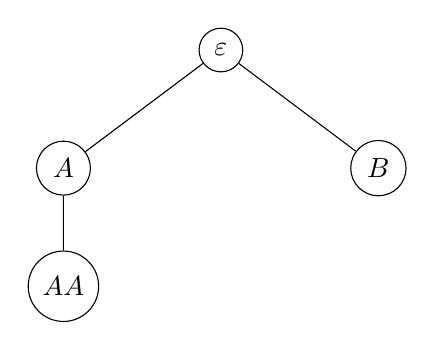
\begin{tikzpicture}[level/.style={sibling distance=40mm/#1}]
	\node [circle,draw] (epsilon){$\varepsilon$}
		child { node [circle,draw] (A) {$A$} 
				child { node[circle,draw](AA){$AA$}  }
			}
		child {node [circle,draw] (B) {$B$} }
	;
	
	\end{tikzpicture}


Como usted puede ver a menor cantidad de símbolos en la sesión estos generan un árbol de menor altura y menos nodos, cada nodo como se ha señalado en el capitulo 4 representa un visita a una sección en particular de la web de MSNBC. Cuando un webaccess posee  pocas secciones o páginas visitadas, la proyección de probabilidades de los posibles símbolos en el alfabeto hace que la probabilidad del siguiente acceso sea equiprobable dentro del los símbolos de nuestro diccionario, de lo anterior convergemos en que mayor es el entrenamiento mejor será la predicción.

Dado el evento $x$  a predecir que pertenece a una secuencia discreta, la probabilidad de $P( x| AB  ) = A $, es el resultado de esta sesión de entrenamiento, pero la probabilidad $P(x | AAB) = ?$, es desconocida.  Si extendemos los símbolos de este nodo cada nodo hijo tendría un probabilidad de $ \dfrac{1}{\Sigma} = \dfrac{1}{17} = 0.0588 $ o bien sería  $\dfrac{1}{ |\sigma| }$, siendo $|\sigma|$ el total de símbolos que se encuentran en el alfabeto. 

Para corroborar este comportamiento haremos distintos experimentos en distintos volúmenes de datos, usaremos una validación cruzada para medir el Accurracy, la cual será nuestra métrica a utilizar.

Con esto demostraremos que secuencias con menores cantidad de símbolos generar un tipo de ruido a la métrica  que afecta en su a nuestra exactitud esperada, cuando hacemos iteraciones de evaluaciones sobre el mayor orden, por otra parte veremos como con una menor cantidad de sesiones de entrenamiento podemos lograr un Accurracy bastante optimista.




\begin{enumerate}
	% Idea de experimento con disminución del tamaño del alfabeto
	\item \label{exp1} \textbf{Experimento con sesiones de usuarios con datos generados de forma sintética}
	
	
	Creamos un set de datos en el cual pudiesemos esperar valores conocidos. Además acotamos a un diccionario de solo tres elementos, el Accurracy obtenido es:
	
	
	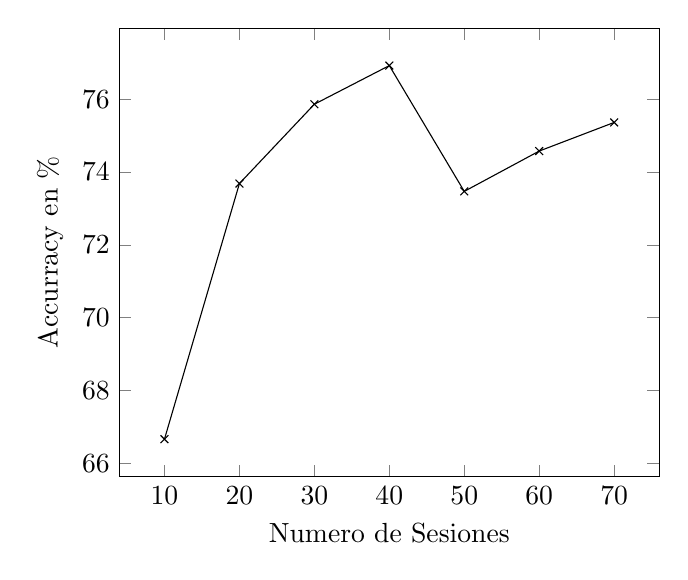
\begin{tikzpicture}
	\begin{axis}[
	xlabel= Numero de Sesiones,
	ylabel=Accurracy en \% ]
	\addplot[color=black,mark=x] coordinates {
		(10, 66.6666666666666)
		(20, 73.6842105263157)
		(30, 75.8620689655172)
		(40, 76.9230769230769)
		(50, 73.469387755102)
		(60, 74.5762711864406)
		(70, 75.3623188405797)
	};
	\end{axis}
	\end{tikzpicture}
	
 
	
	En el gráfico anterior usamos como mínimo 10 sesiones de las 80 de disponibles que se usaron par este experimento. Dado a que en este caso la cantidad de sesiones es bien reducida y cada símbolo posee una gran frecuencia existe mayor redundancia de datos y nuestro modelo se comporta como espera que lo haga un algoritmo de compresión de datos. Entre mayor es la cantidad de símbolos iguales
	que van entrenando al \emph{LZtrie}, hay una aglomeración de frecuencia en ciertos nodos, pero estos son minimizados por los niveles que genera al momento de la construcción del árbol.
	
	La tasa de frecuencia de un símbolo converge a predicciones de secuencias evaluadas que caen en el nodo con mejor probabilidad dado $\epsilon$ (Raiz del \emph{trie}).
	


	\newcommand{\slice}[4]{
		\pgfmathparse{0.5*#1+0.5*#2}
		\let\midangle\pgfmathresult
		
		% slice
		\draw[thick,fill=black!10] (0,0) -- (#1:1) arc (#1:#2:1) -- cycle;
		
		% outer label
		\node[label=\midangle:#4] at (\midangle:1) {};
		
		% inner label
		\pgfmathparse{min((#2-#1-10)/110*(-0.3),0)}
		\let\temp\pgfmathresult
		\pgfmathparse{max(\temp,-0.5) + 0.8}
		\let\innerpos\pgfmathresult
		\node at (\midangle:\innerpos) {#3};
	}
	
	\begin{center}
	\begin{tikzpicture}[scale=1.5]
	
	\newcounter{a}
	\newcounter{b}
	\foreach \p/\t in {61.5/page A, 35.9/page B, 12.8/type C }
	{
		\setcounter{a}{\value{b}}
		\addtocounter{b}{\p}
		\slice{\thea/100*360}
		{\theb/100*360}
		{\p\%}{\t}
	}
	
	\end{tikzpicture}
	\end{center}
	

	Tal como se puede ver en el gráfico anterior existe un gran probabilidad de que dado una secuencia de accesos después de $\epsilon$ la próxima sección a acceder sea la página A.
	Esto es adicionalmente es consistente a el tipo de set de datos que hemos ocupado ya que con esto podemos delimitar a que nuestro modelo al tener símbolos bastante frecuente no crea un trie desbalanceado, para este caso solo acota constantemente a un altura de 5 niveles y una variación mínima entre la exactitud, que posee el entrenamiento versus set de evaluaciones, incluso podemos solo podemos usar un entrenamiento de por lo menos 30 sesiones para predecir 50 sesiones con un Accurracy con un margen de error máximo de $10\%$ en el peor de los casos. 
	Lo anterior si lo comparamos con un evento aleatorio como resultado nos daría que nuestro modelo es bastante mejor que una predicción aleatoria, es decir $ 66.7\%  \geq 33\%$, siendo esta una comparativa optimista de que al menos nuestro modelo dado un set de datos artificial.
	
	
	
	

	\item 
	\textbf{Sesiones con menor redundancia y secuencias de largo variable }
	

	Validaremos ahora el comportamiento de nuestro modelo con datos reales con secuencias discretas distribuidas no uniformemente.
	
	
	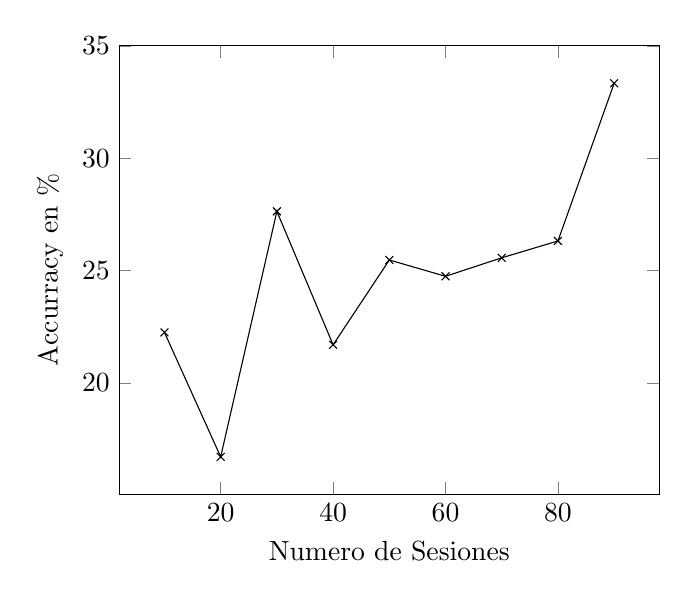
\begin{tikzpicture}
		\begin{axis}[
		xlabel= Numero de Sesiones,
		ylabel=Accurracy en \% ]
		\addplot[color=black,mark=x] coordinates {
			(10, 22.2471910112359)
			(20, 16.7088607594936)
			(30, 27.6328502415459)
			(40, 21.6949152542372)
			(50, 25.469387755102)
			(60, 24.7435897435897)
			(70, 25.5665024630541)
			(80, 26.3157894736842)
			(90, 33.3333333333333)
		};
		\end{axis}
	\end{tikzpicture}
		

	En este caso si existe una menor redundancia a diferencia del experimento \ref{exp1} lo que produce que el modelo tengo un rendimiento bajo, aún así dada sigue siendo en el mejor de los casos seis veces mejor que la probabilidad aleatoria de predecir. En este experimento usamos un $|\sigma| =15$, por ende tenemos que dado nuestro modelo, 
	
	\begin{equation}\label{expResult2}
		M( x | \mbox{90\% train}  ) = 33 \% \geq M( x | \mbox{random}  ) = 6.66\% 
	\end{equation}, como hemos visto en (\ref{expResult2}) nuestro modelo sigue siendo válido en un escenario en que los datos se dispersan considerablemente. 
	Adicionalmente en este tipo de caso existe un comportamiento de nuestro modelo en el cual hace el mejor esfuerzo por mantener la compresibilidad de los datos mayor o igual a la predictibilidad del mismo, peor al tener mayor dispersión la altura para una cantidad similar de sesiones en (\label{expResult2}) sigue siendo 5. Pero la cantidad de nodos sufre un gran incremento, podemos verlo en:
	
	
	
	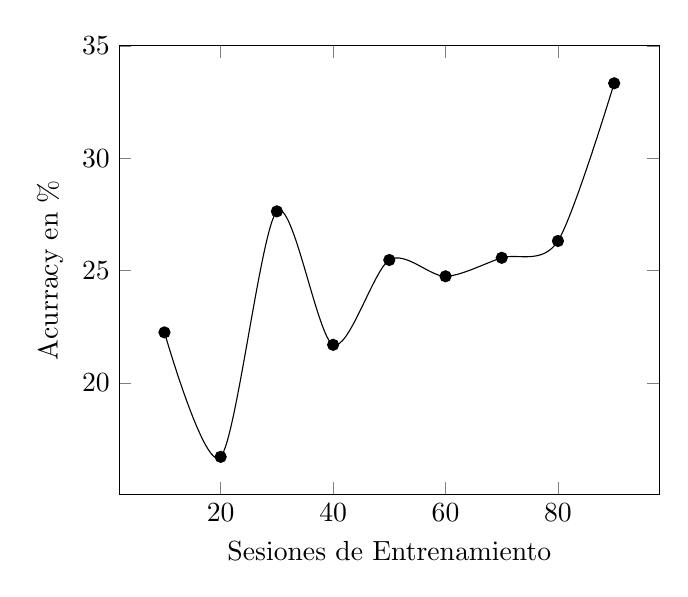
\begin{tikzpicture}
	\begin{axis}[
	xlabel=$\mbox{Sesiones de Entrenamiento}$,
	ylabel=$\mbox{Acurracy en \%}$]
	\addplot[smooth,mark=*,black] plot coordinates {
			(10, 22.2471910112359)
			(20, 16.7088607594936)
			(30, 27.6328502415459)
			(40, 21.6949152542372)
			(50, 25.469387755102)
			(60, 24.7435897435897)
			(70, 25.5665024630541)
			(80, 26.3157894736842)
			(90, 33.3333333333333)
	};

	
%	\addplot[smooth,color=red,mark=x]
%	plot coordinates {
%			(10, 10)
%			(20, 10)
%			(30, 10)
%			(40, 10)
%			(50, 19)
%			(60, 33)
%			(70, 56)
%			(80, 66)
%			(90, 69)
%	};
%	\addlegendentry{Nodes/train}
	\end{axis}
	\end{tikzpicture}


	Acorde al gráfico anterior podemos señalar que al haber un incremento en la dispersión de los datos y menor redundancia, el crecimiento de nuestro árbol será horizontal, ya que para tanto como hemos en este experimento y en (\label{expResult2}), la altura del nodo no tiene una relación directa a la redundancia ó dispersión, pero si a la cantidad de sesiones evaluadas. 
	
	Además, al mayor esfuerzo que hace el predictor por lograr mejores resultados se construyen mas nodos, por lo que el modelo LDC, deja de comprimir por satisfacer las condiciones de predictibilidad necesarias para seguir siendo válido.

	
	Iteramos una nueva evaluación con las mismas condiciones pero subiendo el volumen de datos de 100 a 1000. Con este buscaremos ver encontrar el mismo comportamiento a un mayor nivel de datos.
	


	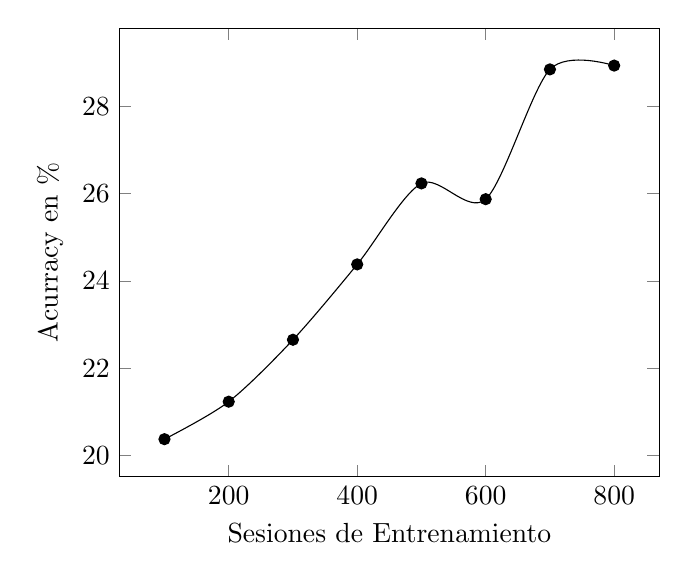
\begin{tikzpicture}
		\begin{axis}[
		xlabel=$\mbox{Sesiones de Entrenamiento}$,
		ylabel=$\mbox{Acurracy en \%}$]
		\addplot[smooth,mark=*,black] plot coordinates {
			(100,  20.3715239154616)
			(200,  21.2302878598247)
			(300,  22.6490224129709)
			(400,  24.3752086811352)
			(500,  26.2308617234469)
			(600,  25.8692564745196)
			(700,  28.8423315814619)
			(800,  28.929431438127)
		};
		\end{axis}
	\end{tikzpicture}
	
	El modelo sigue siendo válido al ir aumentando el volumen de datos bajo las mismas circunstancias. Incluso para ambos experimentos anteriores podemos sacar la relación que nuestro modelo posee una tasa de error de $\pm4\%$ al aumentar 100 veces con respecto a la primera iteración de este escenario cuando se usa la  mayor cantidad de sesiones de entrenamiento posible.


	Otra particularidad que ha demostrado el modelo gracias a las propiedades de compresibilidad de Lempel Ziv\cite{ZivLempel1977} es la Minimización de niveles requeridos aún cuando la cantidad de nodos va creciendo.
	
	
	
	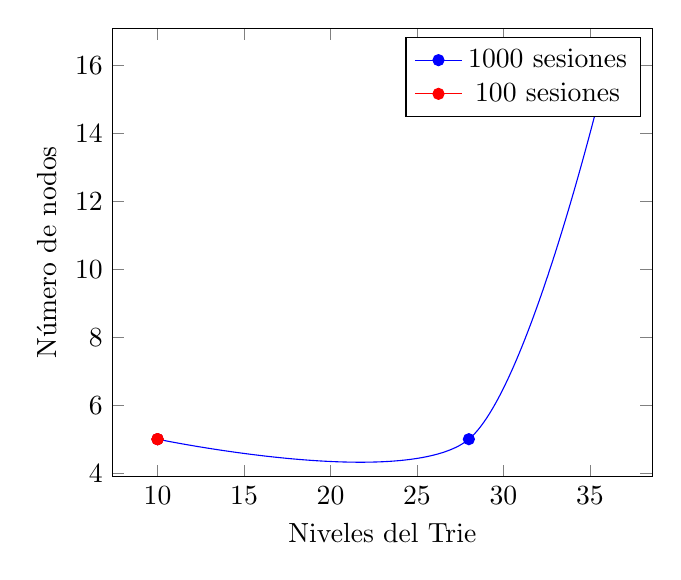
\begin{tikzpicture}
	\begin{axis}[
	xlabel=$\mbox{Niveles del Trie}$,
	ylabel=$\mbox{Número de nodos}$]
	\addplot[smooth,mark=*,blue] plot coordinates {
		( 10,5 )
		(  28 ,5)
		( 36 , 16)

	};

	\addlegendentry{ 1000 sesiones }

	\addplot[smooth,mark=*,red] plot coordinates {
		( 10,5 )
		( 10,5 )
		( 10,5 )
	};
	\addlegendentry{ 100 sesiones }
	
	\end{axis}
	\end{tikzpicture}


	Como podemos ver en el comportamiento de inicio del modelo el criterio de partida en el escenario descrito es compartido por ambos experimentos.



	También dado a que este no es uno de los casos más favorables para nuestro modelo de predictivo, podriamos tener un diferencial en los tiempos de construcción del Trienode acorde a la cantidad de nodos necesarios para los criterios de entrenamiento, 


	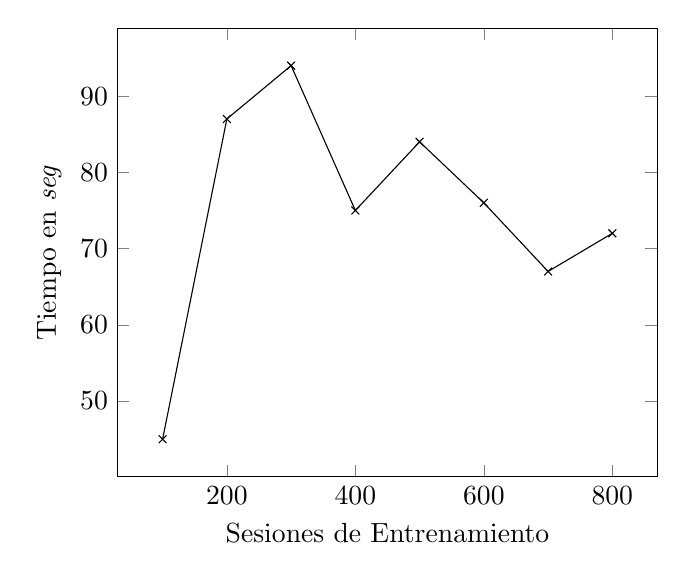
\begin{tikzpicture}
	\begin{axis}[
	xlabel= Sesiones de Entrenamiento ,
	ylabel=Tiempo en \emph{seg} ]
	\addplot[color=black,mark=x] coordinates {
			(100, 45 )
			(200, 87 )
			(300, 94 )
			(400, 75 )
			(500, 84 )
			(600, 76 )
			(700, 67)
			(800, 72 )
	};
	\end{axis}
	\end{tikzpicture}





	\item \label{exp4}	
	\textbf{Sesiones con tamaño de secuencia constante}

	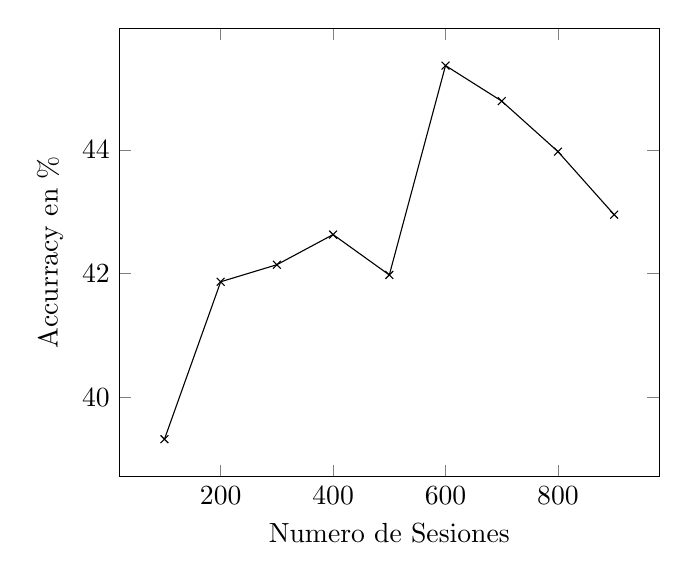
\begin{tikzpicture}
	\begin{axis}[
	xlabel= Numero de Sesiones,
	ylabel=Accurracy en \% ]
	\addplot[color=black,mark=x] coordinates {
			(100, 39.3259176863181 )
			(200, 41.8698372966207 )
			(300, 42.1454458750596 )
			(400, 42.6323038397328 )
			(500, 41.9799599198396 )
			(600, 45.3634085213033 )
			(700, 44.7892976588628)
			(800, 43.9736180904522 )
			(900, 42.9539842873176 )
	};
	\end{axis}
	\end{tikzpicture}

	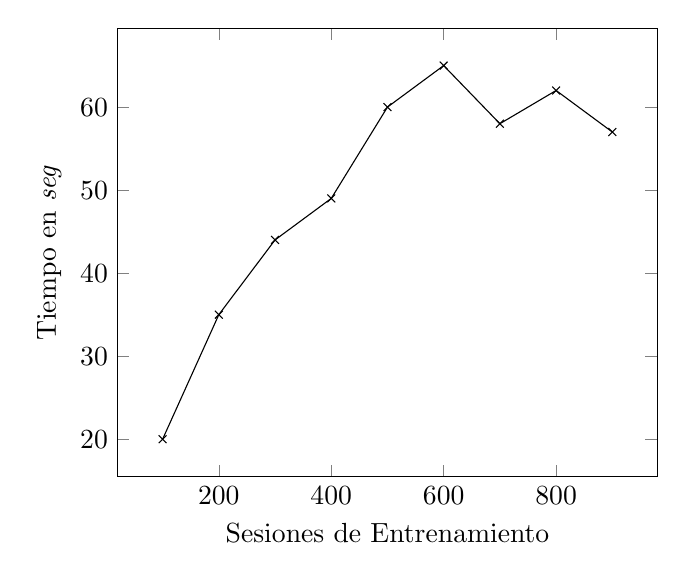
\begin{tikzpicture}
	\begin{axis}[
	xlabel= Sesiones de Entrenamiento ,
	ylabel=Tiempo en \emph{seg} ]
	\addplot[color=black,mark=x] coordinates {
			(100, 20)
			(200, 35)
			(300, 44)
			(400, 49)
			(500, 60)
			(600, 65)
			(700, 58)
			(800, 62)
			(900, 57 )
	};
	\end{axis}
	\end{tikzpicture}





	\item \label{exp5}
		
	\textbf{Sesiones de acceso con cota inferior 100 símbolos }
	
	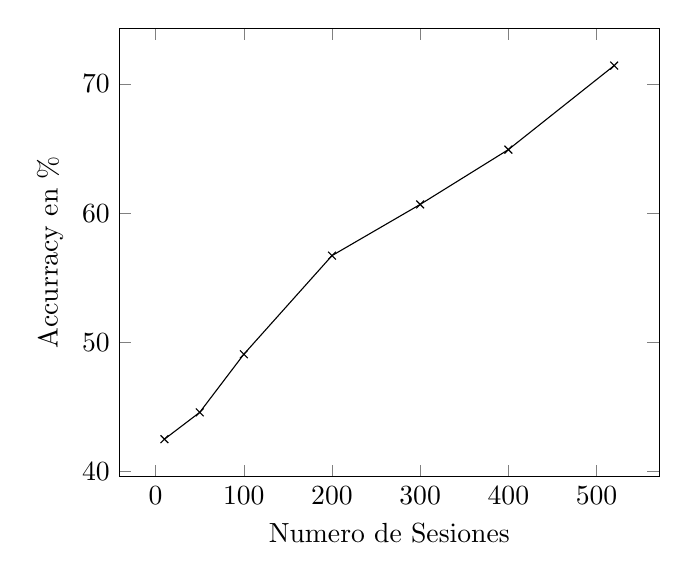
\begin{tikzpicture}
	\begin{axis}[
	xlabel= Numero de Sesiones,
	ylabel=Accurracy en \% ]
	\addplot[color=black,mark=x] coordinates {
		(10 ,  42.5190839694656 )
		(50 ,  44.595041322314 )
 		(100 , 49.089861751152 )
 		(200 , 56.7230538922155 )
 		(300 , 60.6837606837608 )
 		(400 , 64.9253731343282 )
 		(520 , 71.4285714285715 )			
	};
	\end{axis}
	\end{tikzpicture}
	
	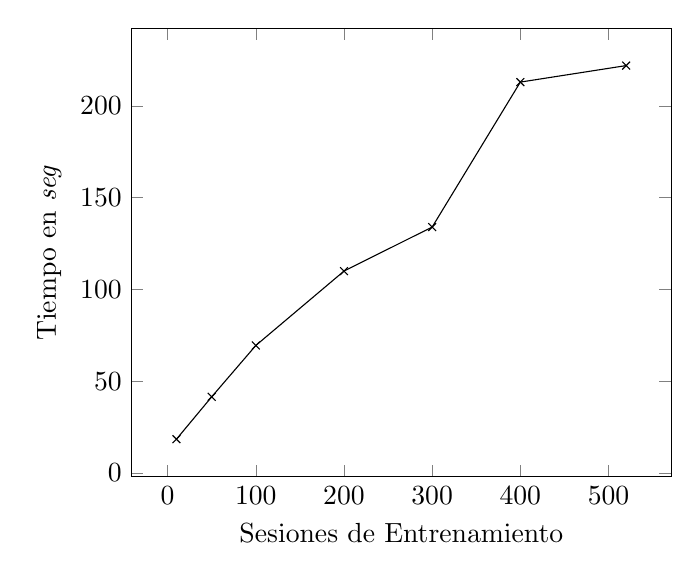
\begin{tikzpicture}
	\begin{axis}[
	xlabel= Sesiones de Entrenamiento ,
	ylabel=Tiempo en \emph{seg} ]
	\addplot[color=black,mark=x] coordinates {
		(10 ,  18.4)
		(50 ,  41.5)
		(100 , 69.46)
		(200 , 110)
		(300 , 134)
		(400 , 213)
		(520 , 222)	
	};
	\end{axis}
	\end{tikzpicture}

	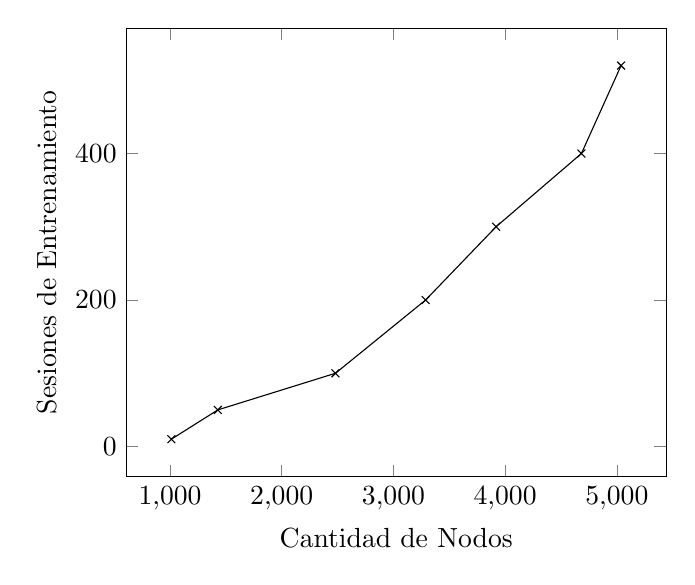
\begin{tikzpicture}
	\begin{axis}[
	xlabel= Cantidad de Nodos,
	ylabel=Sesiones de Entrenamiento  ]
	\addplot[color=black,mark=x] coordinates {
		(1012,10 )
		(1428,50 )
		(2481,100 )
		(3288,200 )
		(3919,300 )
		(4683,400 )
		(5038,520 )	
	};
	
 	
	\end{axis}
	\end{tikzpicture}	


	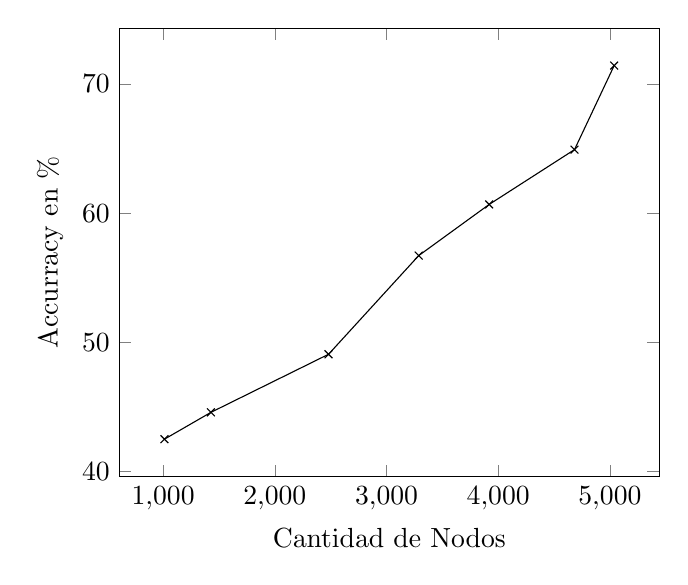
\begin{tikzpicture}
	\begin{axis}[
	xlabel=Cantidad de Nodos,
	ylabel=Accurracy en \%  ]
 
	\addplot[color=black,mark=x] coordinates {
		(1012,42.5190839694656 )
		(1428,44.595041322314 )
		(2481,49.089861751152 )
		(3288,56.7230538922155 )
		(3919,60.6837606837608 )
		(4683,64.9253731343282 )
		(5038,71.4285714285715 )	
	};	
	\end{axis}
	\end{tikzpicture}

	
	
	
	
	\item \label{exp6}	
	\textbf{Sesiones con menos de 5 webaccess para generar el Trie}
	
	
	
	Hacemos una validación cruzada para una muestra de data de 906130 sesiones de usuarios para probar como se comporta con cross validation.
	
	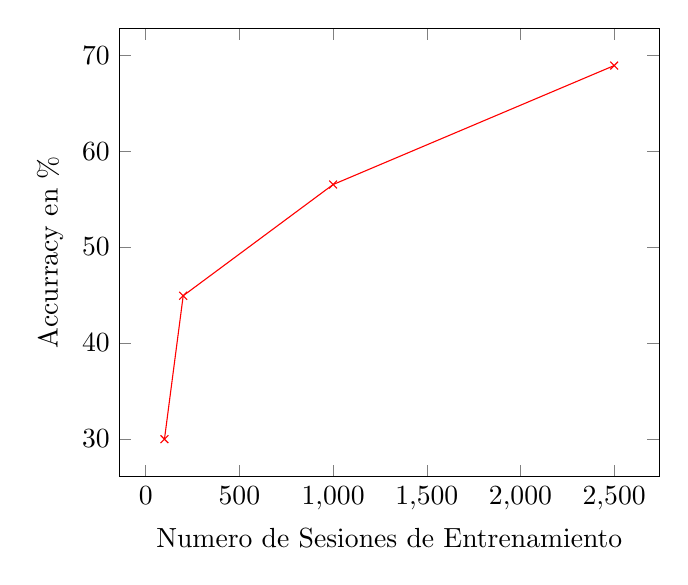
\begin{tikzpicture}
	\begin{axis}[
	xlabel= Numero de Sesiones de Entrenamiento,
	ylabel=Accurracy en \% ]
	\addplot[color=red,mark=x] coordinates {
		(100, 29.9674371114825)
		(200, 44.9237667712101)
		(1000, 56.519572924979)
		(2500, 68.9237667712101)
 
	};
	\end{axis}
	\end{tikzpicture}
	
	
	
	
	
	
	
	
	
	
	
	
	
	
	
	
	
	\item  Dataset uniformes de largo acotado inferiormente y volumenes de alto tamaño.


	
\end{enumerate}








 



	% \begin{forest} 
	% 	[VP
	% 	[DP]
	% 	[V’
	% 	[V]
	% 	[DP]
	% 	]
	% 	]
	% \end{forest}



	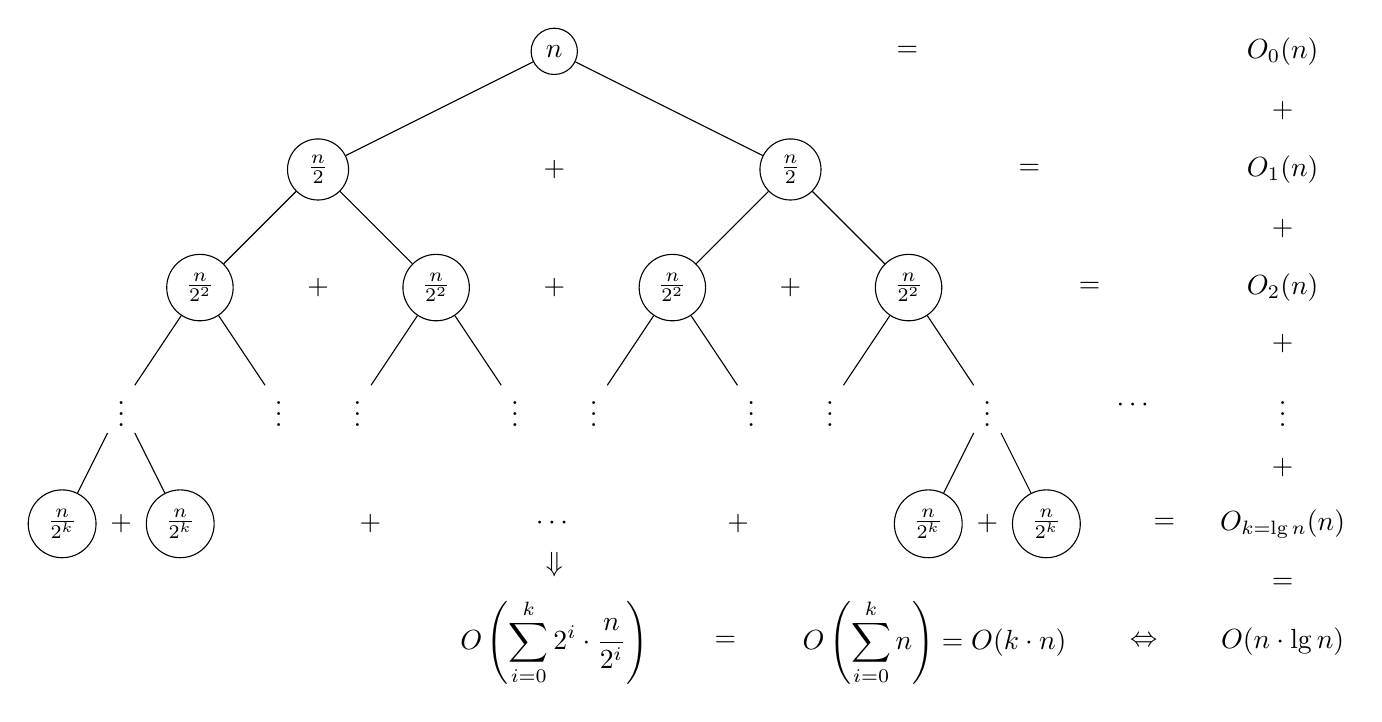
\begin{tikzpicture}[level/.style={sibling distance=60mm/#1}]
	\node [circle,draw] (z){$n$}
	child {node [circle,draw] (a) {$\frac{n}{2}$}
		child {node [circle,draw] (b) {$\frac{n}{2^2}$}
			child {node {$\vdots$}
				child {node [circle,draw] (d) {$\frac{n}{2^k}$}}
				child {node [circle,draw] (e) {$\frac{n}{2^k}$}}
			} 
			child {node {$\vdots$}}
		}
		child {node [circle,draw] (g) {$\frac{n}{2^2}$}
			child {node {$\vdots$}}
			child {node {$\vdots$}}
		}
	}
	child {node [circle,draw] (j) {$\frac{n}{2}$}
		child {node [circle,draw] (k) {$\frac{n}{2^2}$}
			child {node {$\vdots$}}
			child {node {$\vdots$}}
		}
		child {node [circle,draw] (l) {$\frac{n}{2^2}$}
			child {node {$\vdots$}}
			child {node (c){$\vdots$}
				child {node [circle,draw] (o) {$\frac{n}{2^k}$}}
				child {node [circle,draw] (p) {$\frac{n}{2^k}$}
					child [grow=right] {node (q) {$=$} edge from parent[draw=none]
						child [grow=right] {node (q) {$O_{k = \lg n}(n)$} edge from parent[draw=none]
							child [grow=up] {node (r) {$\vdots$} edge from parent[draw=none]
								child [grow=up] {node (s) {$O_2(n)$} edge from parent[draw=none]
									child [grow=up] {node (t) {$O_1(n)$} edge from parent[draw=none]
										child [grow=up] {node (u) {$O_0(n)$} edge from parent[draw=none]}
									}
								}
							}
							child [grow=down] {node (v) {$O(n \cdot \lg n)$}edge from parent[draw=none]}
						}
					}
				}
			}
		}
	};
	\path (a) -- (j) node [midway] {+};
	\path (b) -- (g) node [midway] {+};
	\path (k) -- (l) node [midway] {+};
	\path (k) -- (g) node [midway] {+};
	\path (d) -- (e) node [midway] {+};
	\path (o) -- (p) node [midway] {+};
	\path (o) -- (e) node (x) [midway] {$\cdots$}
	child [grow=down] {
		node (y) {$O\left(\displaystyle\sum_{i = 0}^k 2^i \cdot \frac{n}{2^i}\right)$}
		edge from parent[draw=none]
	};
	\path (q) -- (r) node [midway] {+};
	\path (s) -- (r) node [midway] {+};
	\path (s) -- (t) node [midway] {+};
	\path (s) -- (l) node [midway] {=};
	\path (t) -- (u) node [midway] {+};
	\path (z) -- (u) node [midway] {=};
	\path (j) -- (t) node [midway] {=};
	\path (y) -- (x) node [midway] {$\Downarrow$};
	\path (v) -- (y)
	node (w) [midway] {$O\left(\displaystyle\sum_{i = 0}^k n\right) = O(k \cdot n)$};
	\path (q) -- (v) node [midway] {=};
	\path (e) -- (x) node [midway] {+};
	\path (o) -- (x) node [midway] {+};
	\path (y) -- (w) node [midway] {$=$};
	\path (v) -- (w) node [midway] {$\Leftrightarrow$};
	\path (r) -- (c) node [midway] {$\cdots$};
	\end{tikzpicture}



%Las conclusiones son deducidas logicamen- te de los resultados obtenidos y de la interpretacionpresen- tada, ademas estan conectadas al marco teorico.
%Las conclusiones muestran el logro de los ob jetivos.
%Se presentan proyec- ciones validas y valio- sas a partir del traba- jo realizado.
%Se detallan claramen- te las limitaciones del traba jo realizado.



\subsection{Detección de Ruido en sesiones}

Al modelar una navegación de usuario mediante un trie basado en un algoritmo como LZ78, adoptamos un enfoque basado en la frecuencia por lo cual si realizamos experimentos para poder encontrar ruido veremos que que son secuencias de acceso comunes y estas no dan relevancia o aportan a la exactitud ó precisión del algoritmo.

Sea la secuencia $\{A,A,A,A,A,A,A,A,A,A,A,A \}$ a la cual llamaremos secuencia $R$, si $A$ es representado por el \emph{home} ó página de inicio, esto da a interpretación que existe un usuario en su sesión $R$ que se encuentra accediendo constantemente a esta sección. Podemos señalar que esta es una sesión ruidosa si:

\begin{equation}
	P( x | AAAAAAA)= A	
\end{equation}, pero siendo la sesión $R$ de tamaño = 12, en el siguiente acceso tendremos una probabilidad equiprobable dentro de las secciones en nuestro alfabeto, la cual generará un probabilidad de éxito ''falso positivo''.

En el siguiente experimento veremos como se comporta nuestro modelo dado entradas \emph{Ruidosas}. Además se mostrará como el árbol suele perder su balance a medida que va creciendo los niveles de altura. 



Por otro lado teniendo la noción de como es el funcionamiento de un servidor IIS, y al ser una página con un gran número de visitas, podemos señalar que los datos proporcionados no son totalmente representativos de usuarios reales, ya que la web al bien indexada en los buscadores existen un cantidad indeterminada de \emph{Crawlers} ó \emph{Bots} que están constantemente generando accesos tanto para almacenar en caché páginas o generando accesos automatizados a ciertos secciones sin ser datos representativo. Dejamos como discusión que algoritmo se podría implementar para detección de estos patrones por las ramas que hemos generado para la detección de \emph{bots} o \emph{robots}



 



%%%%%%%%%%%%%%%%%%%%%%%%%%%%%%%%%%%%%%%%%%%%%%%% APUNTES
%%%%%%%%  haciendo prubeas con crosss validate con  80 t y 20 de eval, consigo peor predicción que con menos data 
%%%%%%%%  Además el arbol  al tener mmás információn, comienza a crecer desmensuaradmente
%%%%%%%% de hecho las mejores predicciones son cunado hay ruido o sesiones repetitivas DATASOURCE >>>penultimate page= A  last page= A  session= AAAAAAAA
%%%%%%%%

 


%%%%%%%%

% 100 datos
% Con sequencias de igual tamaño (sesiones con un número de accesos > 5 ) llego a una accurracy del 28.3% con 10t y 90 eval
% Con sequencias de igual tamaño (sesiones con un número de accesos > 5 ) llego a una accurracy del 19.2% con 20t y 80 eval
% Con sequencias de igual tamaño (sesiones con un número de accesos > 5 ) llego a una accurracy del 18.4% con 30t y 70 eval
% Con sequencias de igual tamaño (sesiones con un número de accesos > 5 ) llego a una accurracy del 21.3% con 40t y 60 eval
% Con sequencias de igual tamaño (sesiones con un número de accesos > 5 ) llego a una accurracy del 17.1% con 50t y 50 eval
% Con sequencias de igual tamaño (sesiones con un número de accesos > 5 ) llego a una accurracy del 14.23% con 70t y 30 eval

% Con sequencias de igual tamaño (sesiones con un número de accesos > 5 ) llego a una accurracy del 18.3% con 90t y 10 eval



% En donde mayor se tienen problemas para las predicciones son en los nodos hojas y nodos intermedios 
% los cuales tienen mas de 3 hijos con probabibilidades equiprobables de acierto


% Los otros casos donde se generan una gran cantidad de errores en las predicciones son secuencias de acceso que son equivalentes a 1 acceso.
% Dado que no hay un historial de la sesión este cae un random dentro de un subconjunto de posibles accesos equiprobables.


%%%%%%%%
%%%%%%%%

Hacemos un experimento con datos totalmente aleatorios de una muestra de 100 acceso
aparte de darle mas diveridad a las sessiones acotamos también a sesiones que por lo menos tengan
3 webaccess 

 

El orden de como se ingresan las sesiones afecta directamente proporcional a la construcción del modelo LZ Trie,
por lo cual es un factor ya que es como un FIFO al momento de crear, lo primero que lee es lo primero que entrena
por lo cual se debise tener un criterior para ordenar los webaccess antes de poder pasarlos al entrenador

@Discusión: Como LZ Trie, es en sí un compresor este no toma decisión, una posible mejora
sería implementar intrinsicamente un Decission tree dentro de subarboles dentro del trie para
poder elegir el más optimo acorde a los criterios historicos, asi podría darse el caso de ser
un compresor-predictor  ``menos tonto''


@Pregunta : ¿Porque se presenta el patron que a menos datos de que tenga el trie mayor es accurracy?

%%%%%%%%
%%%%%%%%






% Idea de experimento con cantidad acotada de nodos
% Idea de experimento con altura paramaetrizada del trieNode
% Gráficos de crecimiento del arbol medida en tiempo ms

%%%%%%%%
%%%%%%%%

















\vspace{2cm}

\section{Conclusiones y Contribuciones}


Aún cuando se presenta varios antecedentes, podemos decir que nuestro modelo ocupa bastante menos memoria pero esto va directamente relacionado el tamaño del trieNode de predicción generado.

%
Aun cuando el trieNode que representa totalmente el modelo de navegación del los usuarios de un sitio web, este no puede generalizar completamente el comportamiento estocástico de los usuarios y/o agentes que acceden a los recursos de MSNBC o un cualquier web en general.

Una de las mayores ventajas de nuestro modelo es que al estar embebido en un servidor de Machine Learning, cada nuevo evento que ingresa para la siguiente nueva ejecución esta estará mejor preparado, podríamos decir que la recolección de data de cada evento en particular nos ayudaría a que nuestro modelo en futuros trabajos vaya aprendiendo mas y más precisamente.


A medida que la altura del árbol va creciendo este genera mayor demora en cuanto a la creación del \emph{LZTrie}
% Pero a mayor altura hay mayor precisión.

Hemos validado que hacer un modelo de navegación de usuarios es un perfecta implementación para el uso de un árbol de la familia de Lempel \& Ziv.

A nuestro modelo le es afectado secuencias de menor tamaño, por lo cual se debe trabajar para hacer un aprendizaje de que momento omitirlo o no. Estas sesiones de bajo número de secuencias genera un bajo porcetaje de accurracy. 


% Cual es el minimo entrenamiento para lograr a Predecir ?

Hemos presentado un modelo liviano el cual puede ser utilizado para predecir secuencias de webaccess en demanda.






%In this paper we studied the empirical performance of a number of prominent prediction algorithms. We focused on prediction settings that are more closely related to those required

%%%%%%%%% On Prediction Using Variable Order Markov Models

%$%%%%%%%%
%%n this paper we studied the empirical performance of a number of prominent prediction algorithms. We focused on prediction settings that are more closely related to those required


%On Prediction Using Variable Order Markov Models
%by machine learning practitioners dealing with discrete sequences.
%However, somewhat surprisingly, the best predictor under the log-loss is not the best classifier. On the contrary, the consistently best protein classifier is based on the mediocre lz-ms predictor! This algo- rithm is a simple modification of the well-known Lempel-Ziv-78 (lz78) prediction algorithm, which can capture VMMs with large contexts. The surprisingly good classification accuracy achieved by this algorithm may be of independent interest to protein analysis research and clearly deserves further investigatio 
% Genero toda las referencias para demostrar el uso de la bibliografía
% No es necesario que utilice este comando en su document
%
%Conclusion of this paper Gopalratnam Cook
%a

lz effectively models sequential processes, and is extremely useful for prediction of processes where events are dependent on the previous event history. This is because of the ability of the algorithm to build an accurate model of the source of the events being generated, a feature inherited from its information theoretic background and the LZ78 text compression algorithm. 
%
The effectiveness of the method for learning a measure of time can also be attributed to fact that ALZ is a strong sequential predictor. The sound theoretical principles on which ALZ is founded also mean that ALZ is an optimal Universal Predictor, and can be used in a variety of prediction scenarios.
%conclusion lcoa
%

Dado que la myora de los predictores funcionan de 
manera offline, uno de los aporte de tener estar estructura de algoritmos como servicios es poder tener un motor de prediccion en linea.





\section{Trabajo Futuro}




% Iniciamos el resto de secciones adicionales al contenido: referencias y apendices
\backmatter

%%Se presenta una revision bibliografica acertada, actual, y exhaustiva (se consulta toda la literatura relevante).
%Presenta y redacta los objetivos, el trabajo realizado, y la validacion de manera detallada. Presenta discusiones detalladas, articuladas, claras, y un buen uso del lenguaje tecnico.
% Bibliografía - El estilo por defecto es IEEE Transactions
\bibliographystyle{ieeetr}
\bibliography{IEEEabrv,referencias}


% Simbología y glosario
% Utilice un paquete para generar símbolos y glosarios.
% Por ejemplo: nomencl (http://texdoc.net/pkg/nomencl)
% Anexos
\appendix

\chapter{Primer anexo}
\label{ch:anexo-a}


Configuraciones para hacer correr IntelliJ con Apache SPARK y Prediction.IO 0.94


\begin{lstlisting}[frame=single,basicstyle=\ttfamily\tiny,]
Main class: io.prediction.workflow.CreateWorkflow

VM options: -Dspark.master=local -Dlog4j.configuration=file:/Users/jguzman/PredictionIO/conf/log4j.properties


Program arguments: --engine-id dummy --engine-version dummy --engine-variant engine.json


io.prediction.workflow.CreateWorkflow
-Dspark.master=local -Dlog4j.configuration=file:/Users/jguzman/PredictionIO/conf/log4j.properties -Dorg.xerial.snappy.lib.name=libsnappyjava.jnilib 
--engine-id dummy --engine-version dummy --engine-variant engine.json



SPARK_HOME=/Users/jguzman/PredictionIO/vendors/spark-1.4.1/bin
PIO_FS_BASEDIR=/Users/jguzman/.pio_store
PIO_FS_ENGINESDIR=/Users/jguzman/.pio_store/engines
PIO_FS_TMPDIR=/Users/jguzman/.pio_store/tmp
PIO_STORAGE_REPOSITORIES_METADATA_NAME=pio_meta
PIO_STORAGE_REPOSITORIES_METADATA_SOURCE=ELASTICSEARCH
PIO_STORAGE_REPOSITORIES_MODELDATA_NAME=pio_model
PIO_STORAGE_REPOSITORIES_MODELDATA_SOURCE=LOCALFS
PIO_STORAGE_REPOSITORIES_APPDATA_NAME=pio_appdata
PIO_STORAGE_REPOSITORIES_APPDATA_SOURCE=ELASTICSEARCH
PIO_STORAGE_REPOSITORIES_EVENTDATA_NAME=pio_event
PIO_STORAGE_REPOSITORIES_EVENTDATA_SOURCE=HBASE
PIO_STORAGE_SOURCES_ELASTICSEARCH_TYPE=elasticsearch
PIO_STORAGE_SOURCES_ELASTICSEARCH_HOSTS=localhost
PIO_STORAGE_SOURCES_ELASTICSEARCH_PORTS=9300
PIO_STORAGE_SOURCES_LOCALFS_TYPE=localfs
PIO_STORAGE_SOURCES_LOCALFS_HOSTS=/Users/jguzman/.pio_store/models
PIO_STORAGE_SOURCES_LOCALFS_PORTS=0
PIO_STORAGE_SOURCES_HBASE_TYPE=hbase
PIO_STORAGE_SOURCES_HBASE_HOSTS=0
PIO_STORAGE_SOURCES_HBASE_PORTS=0


Main class: io.prediction.workflow.CreateServer
Program Arguments: --engineInstanceId **replace_with_the_id_from_pio_train**




Try -- for more information.
Usage: pio train [--batch <value>] [--skip-sanity-check]
                 [--stop-after-read] [--stop-after-prepare]
                 [--engine-factory <value>] [--engine-params-key <value>]
                 [--scratch-uri <value>]
                 [common options...]

Kick off a training using an engine (variant) to produce an engine instance.
This command will pass all pass-through arguments to its underlying spark-submit
command.

  --batch <value>
      Batch label of the run.
  --skip-sanity-check
      Disable all data sanity check. Useful for speeding up training in
      production.
  --stop-after-read
      Stop the training process after DataSource.read(). Useful for debugging.
  --stop-after-prepare
      Stop the training process after Preparator.prepare(). Useful for
      debugging.
  --engine-factory
      Override engine factory class.
  --engine-params-key
      Retrieve engine parameters programmatically from the engine factory class.
  --scratch-uri
      URI of the working scratch space. Specify this when you want to have all
      necessary files transferred to a remote location. You will usually want to
      specify this when you use --deploy-mode cluster.

\end{lstlisting}

\vspace{1cm}

Como hacer llamadas curl desde la consola o terminal Linux


\begin{lstlisting}

curl -H "Content-Type: application/json"  -d '{"webaccess" : "AC","num" : 10}' http://52.33.180.212:8000/queries.json



\end{lstlisting}





%\blindtext[5]


\chapter{Segundo anexo}
\label{ch:anexo-b}


%\blindtext[10]


 % Aca se incluyen los archivos con el texto de los anexos


\clearpage
\printglossary[type=\acronymtype]
\printglossary
\end{document}